% !TeX spellcheck = pl_PL
%%%%%%%%%%%%%%%%%%%%%%%%%%%%%%%%%%%%%%%%%%%
%                                        %
% Szablon pracy dyplomowej inzynierskiej %
% zgodny  z aktualnymi  przepisami  SZJK %
%                                        %
%%%%%%%%%%%%%%%%%%%%%%%%%%%%%%%%%%%%%%%%%%
%                                        %
%  (c) Krzysztof Simiński, 2018-2023     %
%                                        %
%%%%%%%%%%%%%%%%%%%%%%%%%%%%%%%%%%%%%%%%%%
%                                        %
% Najnowsza wersja szablonów jest        %
% podstępna pod adresem                  %
% github.com/ksiminski/polsl-aei-theses  %
%                                        %
%%%%%%%%%%%%%%%%%%%%%%%%%%%%%%%%%%%%%%%%%%
%
%
% Projekt LaTeXowy zapewnia odpowiednie formatowanie pracy,
% zgodnie z wymaganiami Systemu zapewniania jakości kształcenia.
% Proszę nie zmieniać ustawień formatowania (np. fontu,
% marginesów, wytłuszczeń, kursywy itd. ).
%
% Projekt można kompilować na kilka sposobów.
%
% 1. kompilacja pdfLaTeX
%
% pdflatex main
% bibtex   main
% pdflatex main
% pdflatex main
%
%
% 2. kompilacja XeLaTeX
%
% Kompilatacja przy użyciu XeLaTeXa różni się tym, że na stronie
% tytułowej używany jest font Calibri. Wymaga to jego uprzedniego
% zainstalowania.
%
% xelatex main
% bibtex  main
% xelatex main
% xelatex main
%
%
%%%%%%%%%%%%%%%%%%%%%%%%%%%%%%%%%%%%%%%%%%%%%%%%%%%%%
% W przypadku pytań, uwag, proszę pisać na adres:   %
%      krzysztof.siminski(małpa)polsl.pl            %
%%%%%%%%%%%%%%%%%%%%%%%%%%%%%%%%%%%%%%%%%%%%%%%%%%%%%
%
% Chcemy ulepszać szablony LaTeXowe prac dyplomowych.
% Wypełniając ankietę spod poniższego adresu pomogą
% Państwo nam to zrobić. Ankieta jest całkowicie
% anonimowa. Dziękujemy!


% https://docs.google.com/forms/d/e/1FAIpQLScyllVxNKzKFHfILDfdbwC-jvT8YL0RSTFs-s27UGw9CKn-fQ/viewform?usp=sf_link
%
%%%%%%%%%%%%%%%%%%%%%%%%%%%%%%%%%%%%%%%%%%%%%%%%%%%%%%%%%%%%%%%%%%%%%%%%%

%%%%%%%%%%%%%%%%%%%%%%%%%%%%%%%%%%%%%%%%%%%%%%%
%                                             %
% PERSONALIZACJA PRACY – DANE PRACY           %
%                                             %
%%%%%%%%%%%%%%%%%%%%%%%%%%%%%%%%%%%%%%%%%%%%%%%

% Proszę wpisać swoje dane w poniższych definicjach.

% TODO
% dane autora
\newcommand{\FirstNameAuthor}{Artur}
\newcommand{\SurnameAuthor}{Stalmach}
\newcommand{\IdAuthor}{296908}   % numer albumu  (bez $\langle$ i $\rangle$)

% drugi autor:
%\newcommand{\FirstNameCoauthor}{Imię}   % Jeżeli jest drugi autor, to tutaj należy podać imię.
%\newcommand{\SurnameCoauthor}{Nazwisko} % Jeżeli jest drugi autor, to tutaj należy podać nazwisko.
%\newcommand{\IdCoauthor}{$\langle$wpisać właściwy$\rangle$}  % numer albumu drugiego autora (bez $\langle$ i $\rangle$)
% Gdy nie ma drugiego autora, należy zostawić poniższe definicje puste, jak poniżej. Gdy jest drugi autor, należy zakomentować te linie.
\newcommand{\FirstNameCoauthor}{} % Jeżeli praca ma tylko jednego autora, to dane drugiego autora zostają puste.
\newcommand{\SurnameCoauthor}{}   % Jeżeli praca ma tylko jednego autora, to dane drugiego autora zostają puste.
\newcommand{\IdCoauthor}{}  % Jeżeli praca ma tylko jednego autora, to dane drugiego autora zostają puste.
%%%%%%%%%%

\newcommand{\Supervisor}{Doktor Inżynier Patryk Grelewicz}     % dane promotora (bez $\langle$ i $\rangle$)
\newcommand{\Title}{Optymalizacja algorytmu sterowania trójfazowym piecem przemysłowym}           % tytuł pracy po polsku
\newcommand{\TitleAlt}{Optimisation of the control algorithm for a three-phase heating unit}                     % thesis title in English
\newcommand{\Program}{Automatyka i Robotyka}            % kierunek studiów  (bez $\langle$ i $\rangle$)
\newcommand{\Specialisation}{Technologie Informacyjne}     % specjalność  (bez $\langle$ i $\rangle$)
\newcommand{\Departament}{Automatyki i Robotyki}        % katedra promotora  (bez $\langle$ i $\rangle$)

% Jeżeli został wyznaczony promotor pomocniczy lub opiekun, proszę go/ją wpisać ...
\newcommand{\Consultant}{} % dane promotora pomocniczego, opiekuna (bez $\langle$ i $\rangle$)
% ... w przeciwnym razie proszę zostawić puste miejsce jak poniżej:
%\newcommand{\Consultant}{} % brak promotowa pomocniczego / opiekuna

% koniec fragmentu do modyfikacji
%%%%%%%%%%%%%%%%%%%%%%%%%%%%%%%%%%%%%%%%%%


%%%%%%%%%%%%%%%%%%%%%%%%%%%%%%%%%%%%%%%%%%%%%%%
%                                             %
% KONIEC PERSONALIZACJI PRACY                 %
%                                             %
%%%%%%%%%%%%%%%%%%%%%%%%%%%%%%%%%%%%%%%%%%%%%%%

%%%%%%%%%%%%%%%%%%%%%%%%%%%%%%%%%%%%%%%%


%%%%%%%%%%%%%%%%%%%%%%%%%%%%%%%%%%%%%%%%%%%%%%%
%                                             %
% PROSZĘ NIE MODYFIKOWAĆ PONIŻSZYCH USTAWIEŃ! %
%                                             %
%%%%%%%%%%%%%%%%%%%%%%%%%%%%%%%%%%%%%%%%%%%%%%%



\documentclass[a4paper,twoside,12pt]{book}
\usepackage[utf8]{inputenc}                                      
\usepackage[T1]{fontenc}  
\usepackage{amsmath,amsfonts,amssymb,amsthm}
\usepackage[british,polish]{babel} 
\usepackage{indentfirst}
\usepackage{xurl}
\usepackage{xstring}
\usepackage{ifthen}
\usepackage{array}
\usepackage{makecell}
\usepackage{multirow}
\usepackage{rotating}



\usepackage{ifxetex}

\ifxetex
	\usepackage{fontspec}
	\defaultfontfeatures{Mapping=tex—text} % to support TeX conventions like ``——-''
	\usepackage{xunicode} % Unicode support for LaTeX character names (accents, European chars, etc)
	\usepackage{xltxtra} % Extra customizations for XeLaTeX
\else
	\usepackage{lmodern}
\fi



\usepackage[margin=2.5cm]{geometry}
\usepackage{graphicx} 
\usepackage{hyperref}
\usepackage{booktabs}
\usepackage{tikz}
\usepackage{pgfplots}
\usepackage{mathtools}
\usepackage{geometry}
\usepackage{subcaption}   % subfigures
\usepackage[page]{appendix} % toc,
\renewcommand{\appendixtocname}{Dodatki}
\renewcommand{\appendixpagename}{Dodatki}
\renewcommand{\appendixname}{Dodatek}

\usepackage{csquotes}
\usepackage[natbib=true,backend=bibtex,maxbibnames=99]{biblatex}  % kompilacja bibliografii BibTeXem
%\usepackage[natbib=true,backend=biber,maxbibnames=99]{biblatex}  % kompilacja bibliografii Biberem
\bibliography{biblio}

\usepackage{ifmtarg}   % empty commands  

\usepackage{setspace}
\onehalfspacing


\frenchspacing



%%%% TODO LIST GENERATOR %%%%%%%%%

\usepackage{color}
\definecolor{brickred}      {cmyk}{0   , 0.89, 0.84, 0.28}

\makeatletter \newcommand \kslistofremarks{\section*{Uwagi} \@starttoc{rks}}
  \newcommand\l@uwagas[2]
    {\par\noindent \textbf{#2:} %\parbox{10cm}
{#1}\par} \makeatother


\newcommand{\ksremark}[1]{%
{%\marginpar{\textdbend}
{\color{brickred}{[#1]}}}%
\addcontentsline{rks}{uwagas}{\protect{#1}}%
}

\newcommand{\comma}{\ksremark{przecinek}}
\newcommand{\nocomma}{\ksremark{bez przecinka}}
\newcommand{\styl}{\ksremark{styl}}
\newcommand{\ortografia}{\ksremark{ortografia}}
\newcommand{\fleksja}{\ksremark{fleksja}}
\newcommand{\pauza}{\ksremark{pauza `--', nie dywiz `-'}}
\newcommand{\kolokwializm}{\ksremark{kolokwializm}}
\newcommand{\cudzyslowy}{\ksremark{,,polskie cudzysłowy''}}

%%%%%%%%%%%%%% END OF TODO LIST GENERATOR %%%%%%%%%%%

\newcommand{\printCoauthor}{%		
    \StrLen{\FirstNameCoauthor}[\FNCoALen]
    \ifthenelse{\FNCoALen > 0}%
    {%
		{\large\bfseries\Coauthor\par}
	
		{\normalsize\bfseries \LeftId: \IdCoauthor\par}
    }%
    {}
} 

%%%%%%%%%%%%%%%%%%%%%
\newcommand{\autor}{%		
    \StrLen{\FirstNameCoauthor}[\FNCoALenXX]
    \ifthenelse{\FNCoALenXX > 0}%
    {\FirstNameAuthor\ \SurnameAuthor, \FirstNameCoauthor\ \SurnameCoauthor}%
	{\FirstNameAuthor\ \SurnameAuthor}%
}
%%%%%%%%%%%%%%%%%%%%%

\StrLen{\FirstNameCoauthor}[\FNCoALen]
\ifthenelse{\FNCoALen > 0}%
{%
\author{\FirstNameAuthor\ \SurnameAuthor, \FirstNameCoauthor\ \SurnameCoauthor}
}%
{%
\author{\FirstNameAuthor\ \SurnameAuthor}
}%

%%%%%%%%%%%% ZYWA PAGINA %%%%%%%%%%%%%%%
% brak kapitalizacji zywej paginy
\usepackage{fancyhdr}
\pagestyle{fancy}
\fancyhf{}
\fancyhead[LO]{\nouppercase{\it\rightmark}}
\fancyhead[RE]{\nouppercase{\it\leftmark}}
\fancyhead[LE,RO]{\it\thepage}


\fancypagestyle{tylkoNumeryStron}{%
   \fancyhf{} 
   \fancyhead[LE,RO]{\it\thepage}
}

\fancypagestyle{bezNumeracji}{%
   \fancyhf{} 
   \fancyhead[LE,RO]{}
}


\fancypagestyle{NumeryStronNazwyRozdzialow}{%
   \fancyhf{} 
   \fancyhead[LE]{\nouppercase{\autor}}
   \fancyhead[RO]{\nouppercase{\leftmark}} 
   \fancyfoot[CE, CO]{\thepage}
}


%%%%%%%%%%%%% OBCE WTRETY  
\newcommand{\obcy}[1]{\emph{#1}}
\newcommand{\english}[1]{{\selectlanguage{british}\obcy{#1}}}
%%%%%%%%%%%%%%%%%%%%%%%%%%%%%

% polskie oznaczenia funkcji matematycznych
\renewcommand{\tan}{\operatorname {tg}}
\renewcommand{\log}{\operatorname {lg}}

% jeszcze jakies drobiazgi

\newcounter{stronyPozaNumeracja}

%%%%%%%%%%%%%%%%%%%%%%%%%%% 
\newcommand{\printOpiekun}[1]{%		

    \StrLen{\Consultant}[\mystringlen]
    \ifthenelse{\mystringlen > 0}%
    {%
       {\large{\bfseries OPIEKUN, PROMOTOR POMOCNICZY}\par}
       
       {\large{\bfseries \Consultant}\par}
    }%
    {}
} 
%
%%%%%%%%%%%%%%%%%%%%%%%%%%%%%%%%%%%%%%%%%%%%%%
 
% Proszę nie modyfikować poniższych definicji!
\newcommand{\Author}{\FirstNameAuthor\ \MakeUppercase{\SurnameAuthor}} 
\newcommand{\Coauthor}{\FirstNameCoauthor\ \MakeUppercase{\SurnameCoauthor}}
\newcommand{\Type}{PROJEKT INŻYNIERSKI}
\newcommand{\Faculty}{Wydział Automatyki, Elektroniki i Informatyki} 
\newcommand{\Polsl}{Politechnika Śląska}
\newcommand{\Logo}{./img/politechnika_sl_logo_bw_pion_pl.pdf}
\newcommand{\LeftId}{Nr albumu}
\newcommand{\LeftProgram}{Kierunek}
\newcommand{\LeftSpecialisation}{Specjalność}
\newcommand{\LeftSUPERVISOR}{PROWADZĄCY PRACĘ}
\newcommand{\LeftDEPARTMENT}{KATEDRA}
%%%%%%%%%%%%%%%%%%%%%%%%%%%%%%%%%%%%%%%%%%%%%%

%%%%%%%%%%%%%%%%%%%%%%%%%%%%%%%%%%%%%%%%%%%%%%%
%                                             %
% KONIEC USTAWIEŃ                             %
%                                             %
%%%%%%%%%%%%%%%%%%%%%%%%%%%%%%%%%%%%%%%%%%%%%%%




%%%%%%%%%%%%%%%%%%%%%%%%%%%%%%%%%%%%%%%%%%%%%%%
%                                             %
% MOJE PAKIETY, USTAWIENIA ITD                %
%                                             %
%%%%%%%%%%%%%%%%%%%%%%%%%%%%%%%%%%%%%%%%%%%%%%%

% Tutaj proszę umieszczać swoje pakiety, makra, ustawienia itd.


 
%%%%%%%%%%%%%%%%%%%%%%%%%%%%%%%%%%%%%%%%%%%%%%%%%%%%%%%%%%%%%%%%%%%%%
% listingi i fragmentu kodu źródłowego 
% pakiet: listings lub minted
% % % % % % % % % % % % % % % % % % % % % % % % % % % % % % % % % % % 

% biblioteka listings
\usepackage{listings}
\lstset{%
morekeywords={string,exception,std,vector},% słowa kluczowe rozpoznawane przez pakiet listings
language=C++,% C, Matlab, Python, SQL, TeX, XML, bash, ... – vide https://www.ctan.org/pkg/listings
commentstyle=\textit,%
identifierstyle=\textsf,%
keywordstyle=\sffamily\bfseries, %\texttt, %
%captionpos=b,%
tabsize=3,%
frame=lines,%
numbers=left,%
numberstyle=\tiny,%
numbersep=5pt,%
breaklines=true,%
escapeinside={@*}{*@},%
}

% % % % % % % % % % % % % % % % % % % % % % % % % % % % % % % % % % % 
% pakiet minted
%\usepackage{minted}

% pakiet wymaga specjalnego kompilowania:
% pdflatex -shell-escape main.tex
% xelatex  -shell-escape main.tex

%\usepackage[chapter]{minted} % [section]
%%\usemintedstyle{bw}   % czarno-białe kody 
%
%\setminted % https://ctan.org/pkg/minted
%{
%%fontsize=\normalsize,%\footnotesize,
%%captionpos=b,%
%tabsize=3,%
%frame=lines,%
%framesep=2mm,
%numbers=left,%
%numbersep=5pt,%
%breaklines=true,%
%escapeinside=@@,%
%}

%%%%%%%%%%%%%%%%%%%%%%%%%%%%%%%%%%%%%%%%%%%%%%%%%%%%%%%%%%%%%%%%%%%%%



%%%%%%%%%%%%%%%%%%%%%%%%%%%%%%%%%%%%%%%%%%%%%%%
%                                             %
% KONIEC MOICH USTAWIEŃ                       %
%                                             %
%%%%%%%%%%%%%%%%%%%%%%%%%%%%%%%%%%%%%%%%%%%%%%%



%%%%%%%%%%%%%%%%%%%%%%%%%%%%%%%%%%%%%%%%


\begin{document}
%\kslistofremarks

\frontmatter

%%%%%%%%%%%%%%%%%%%%%%%%%%%%%%%%%%%%%%%%%%%%%%%
%                                             %
% PROSZĘ NIE MODYFIKOWAĆ STRONY TYTUŁOWEJ!    %
%                                             %
%%%%%%%%%%%%%%%%%%%%%%%%%%%%%%%%%%%%%%%%%%%%%%%


%%%%%%%%%%%%%%%%%%  STRONA TYTUŁOWA %%%%%%%%%%%%%%%%%%%
\pagestyle{empty}
{
	\newgeometry{top=1.5cm,%
		bottom=2.5cm,%
		left=3cm,
		right=2.5cm}

	\ifxetex
		\begingroup
		\setsansfont{Calibri}

	\fi
	\sffamily
	\begin{center}
		\includegraphics[width=50mm]{\Logo}


		{\Large\bfseries\Type\par}

		\vfill  \vfill

		{\large\Title\par}

		\vfill

		{\large\bfseries\Author\par}

		{\normalsize\bfseries \LeftId: \IdAuthor}

		\printCoauthor

		\vfill

		{\large{\bfseries \LeftProgram:} \Program\par}

		{\large{\bfseries \LeftSpecialisation:} \Specialisation\par}

		\vfill  \vfill 	\vfill 	\vfill 	\vfill 	\vfill 	\vfill

		{\large{\bfseries \LeftSUPERVISOR}\par}

		{\large{\bfseries \Supervisor}\par}

		{\large{\bfseries \LeftDEPARTMENT\ \Departament} \par}

		{\large{\bfseries \Faculty}\par}

		\vfill  \vfill


		\printOpiekun{\Consultant}

		\vfill  \vfill

		{\large\bfseries  Gliwice \the\year}

	\end{center}
	\ifxetex
		\endgroup
	\fi
	\restoregeometry
}

%%%%%%%%%%%%%%%%%%%%%%%%%%%%%%%%%%%%%%%%%%%%%%%
%                                             %
% KONIEC STRONY TYTUŁOWEJ                     %
%                                             %
%%%%%%%%%%%%%%%%%%%%%%%%%%%%%%%%%%%%%%%%%%%%%%%  


\cleardoublepage

\rmfamily\normalfont
\pagestyle{empty}


%%% No to zaczynamy pisać pracę :-) %%%%

% TODO
\subsubsection*{Tytuł pracy}
\Title

\subsubsection*{Streszczenie}
Zakres pracy obejmuje przykładowe podejście do problemu optymalizacji algorytmu sterowania układu automatyki, której celem jest zmniejszenie zużycia urządzeń wykonawczych, przy zachowaniu określonej efektywności pracy, układu regulacji. Rozważanym układem jest instalacja cieplna, służąca do podgrzewania cieczy. Najważniejszy element układu stanowi elektryczny piec przepływowy, wyposażony w trzy grzałki. Grzałki zasilane są za pomocą przekaźników, stanowiących wspomniane elementy wykonawcze. To własnie znaczące zmniejszenie zużycia przekaźników (zmniejszenie liczby przełączeń) jest głównym celem algorytmu. Cel osiągnięto poprzez niezależne sterowanie grzałkami, za pomocą wykorzystania idei systemu trójfazowego. Klasyczne sterowanie, będące jednocześnie punktem odniesienia do tworzonego algorytmu, jest bowiem realizowane w trybie jednofazowym.

\subsubsection*{Słowa kluczowe}
sterowanie, optymalizacja, algorytm, piec, regulacja

\subsubsection*{Thesis title}
\begin{otherlanguage}{british}
	\TitleAlt
\end{otherlanguage}

\subsubsection*{Abstract}
\begin{otherlanguage}{british}
	The scope of the work includes an exemplary approach to the problem of optimising the control algorithm of an automation system, in order to reduce conspumption of the actuators, while maintaining specified control system efficiency. The system under consideration is a thermal installation for heating liquids. The most important part of the system is the electric flow furnace, equipped with three heaters. The heaters are powered by contactors, which are the mentioned actuators. It is the significant reduction in contactor usage (reduction in the number of switchovers) that is the main objective of the algorithm. The objective was achieved by controlling the heaters independently, using the idea of a three-phase system. This is because the classic control, which is also the reference point for the algorithm being developed, is implemented in single-phase mode.
\end{otherlanguage}
\subsubsection*{Key words}
\begin{otherlanguage}{british}
	control, optimisation, algorithm, furnance, regulation
\end{otherlanguage}




%%%%%%%%%%%%%%%%%% SPIS TRESCI %%%%%%%%%%%%%%%%%%%%%%
% Add \thispagestyle{empty} to the toc file (main.toc), because \pagestyle{empty} doesn't work if the TOC has multiple pages
\addtocontents{toc}{\protect\thispagestyle{empty}}
\tableofcontents

%%%%%%%%%%%%%%%%%%%%%%%%%%%%%%%%%%%%%%%%%%%%%%%%%%%%%
\setcounter{stronyPozaNumeracja}{\value{page}}
\mainmatter
\pagestyle{empty}

\cleardoublepage

\pagestyle{NumeryStronNazwyRozdzialow}

%%%%%%%%%%%%%% TREŚĆ PRACY %%%%%%%%%%%%%%%%%

% TODO
\chapter{Wstęp}
\label{ch:01}

Efektywność produkcji odgrywa w przemyśle kluczową rolę, w kontekście generowania zysków. Wysoka efektywność produkcji może być osiągana na wiele sposobów. Jednym z ważnych aspektów, w odniesieniu do pojęcia wydajności, jest minimalizowanie strat związanych z procesem produkcyjnym. Przykładem takiego działania może być minimalizowanie zużycia elementów wykonawczych. To zagadnienie zostało w znaczącym stopniu rozwiązane, dzięki rozwojowi automatycznych układów regulacji. Układy regulacji są powszechnie stosowane w przemyśle, ze względu na ich uniwersalne podejście do problemu sterowania procesem oraz prostotę i powszechność implementacji. Stosowanie sprawnych algorytmów sterowania jest niemniej ważne. Tu dziedzina automatyki również oferuje wiele gotowych rozwiązań, jednak opracowanie właściwego algorytmu, wymaga często zastosowania bardziej specyficznego podejścia, w odniesieniu do konkretnego problemu.

\subsection{Pojęcie regulacji w przemyśle}
Układy regulacji są powszechnie obecne we wspołczesnym przemyśle, ponieważ odgrywaja kluczową rolę w utrzymaniu stabilnej i optymalnej pracy, systemów różnego przeznaczenia. Pozwalają one na zautomatyzowanie procesu sterowania, poprzez ciągłe monitorowanie i utrzymywanie wartości określonych parametrów, na odpowiednim poziomie. Takie podejście pozwala na osiągnięcie wysokiej precyzji sterowania procesem, co przekłada się na zwiększenie ogólnej efektywności pracy, bądź jakości produktu końcowego, dzięki znaczącej poprawie następujących (przykładowych) aspektów:

\begin{itemize}
	\item \textbf{Szybka adaptacja}: Obecność układów regulacji w procesach produkcyjnych, pozwala na szybsze dostosowanie istniejących systemów, do nowych warunków produkcyjnych, wymagań branży oraz przepisów.
	\item \textbf{Wydajność}: Możliwość automatyczngo i ciągłego dostosowywania parametrów do zmiennych warunków, pozwala na utrzymywanie jakości procesu na pożądanym poziomie.
	\item \textbf{Zużycie energii}: Możliwość błyskawicznej reakcji na zmienne warunki pracy, pozwala na osiąganie wysokiej efektywności energetycznej.
	\item \textbf{Zmniejszenie kosztów}: Optymalizacja procesów wpływa pozytywnie na minimalizację błedów produkcyjnych oraz zużycia urządzeń i materiałów, co przyczynia się do obniżenia kosztów produkcji i magazynowania.
	\item \textbf{Bezpieczeństwo}: Zwłaszcza w procesach, w których obecne są niebezpieczne substancje, bądź zachodzą procesy chemiczne, ciągła kontrola parametrów odgrywa istotną rolę w zwiększaniu bezpieczeństwa, poprzez minimalizowanie szans na wystąpienie zagrożenia i szybkie reagowanie na zdarzenia losowe. Regulacja nie jest również bez znaczenia, w kontekście problemu redukcji emisji substancji szkodliwych i zanieczyszczeń, do środowiska.
\end{itemize}

\subsubsection{Struktura układu regulacji}
Układami automatycznej regulacji nazywamy układy, składajace się z obiektu regulacji, regulatora oraz elementów automatyki (urządzenia pomiarowe, wykanowacze). Ogólna zasada działania regulatora polega na ciągłym korygowaniu sygnału sterującego, na podstawie monitorowania różnicy (uchybu regulacji) pomiędzy wartością zadaną (pożądaną), a wartością regulowaną (wyjściową). Ogólne działanie układu regulacji można zobrazować za pomocą schematu blokowego, zamieszczonego poniżej.

\begin{figure}[h]
	\centering
	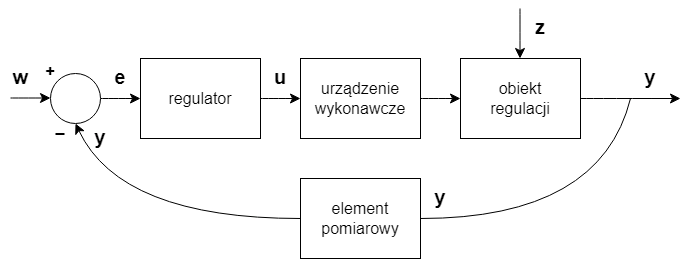
\includegraphics[width=0.8\textwidth]{./img/regulacja.png}
	\caption{Schemat blokowy układu regulacji}
	\label{fig:regulacja}
\end{figure}

\noindent Opis oznaczeń:
\begin{description}
	\item[\textbf{w}:]wartość zadana - wartość, do której dąży wartość regulowana
	\item[\textbf{y}:]wartość regulowana - wartość rzeczywista, która dąży do wartości zadanej
	\item[\textbf{e}:]uchyb regulacji - różnica pomiędzy wartością zadaną, a regulowaną
	\item[\textbf{u}:]wartość sterująca - sygnał przekazywany przez regulator, do urządzeń wykonawczych
	\item[\textbf{z}:]zakłócenia - sygnały wywierające niekorzystny wpływ na wartość regulowaną
\end{description}

\newpage
\subsubsection{Wybór rodzaju regulatora}
W zależności od natury wielkości regulowanej, w przemyśle stosuje się wiele różnych typów regulatorów \cite{chuong2017identification, han2009pid, laszczyk2013comparison}, jednak regulator PID (ang. proportional-integral-derivative) jest w praktyce najczęściej stosowanym rodzajem. Na model matematyczny regulatora PID składają się trzy człony obliczeniowe:

\begin{itemize}
	\item \textbf{Człon P (proporcjonalny)} jest odpowiedzialny za reakcję proporcjonalną do aktualnego błędu regulacji. Im większa różnica pomiędzy wartością zadaną, a rzeczywistą, tym większa siła korygująca.
	\item \textbf{Człon I (całkujący)} jest odpowiedzialny za eliminację błędów statycznych, poprzez akumulację całkowitego błędu w czasie (błędów z przeszłości) i wprowadzanie, na tej podstawie, odpowiedniej korekty.
	\item \textbf{Człon D (różniczujący)} dostarcza korektę na podstawie szybkości zmian błędu regulacji. Skuteczny w układach, gdzie istotne jest sprawne reagowanie na szybkie zmiany. Pozwala na przyspieszenie układu, zwłaszcza wtedy, gdy obiekt regulowany charakteryzuje dynamika wyższego rzędu.
\end{itemize}

\noindent Zasadę działania regulatora PID, który będzie istotnym elementem w kontekście weryfikacji wyników optymalizacji, można zobrazować za pomocą uproszczonego schematu, zamieszczonego poniżej.

\begin{figure}[h]
	\centering
	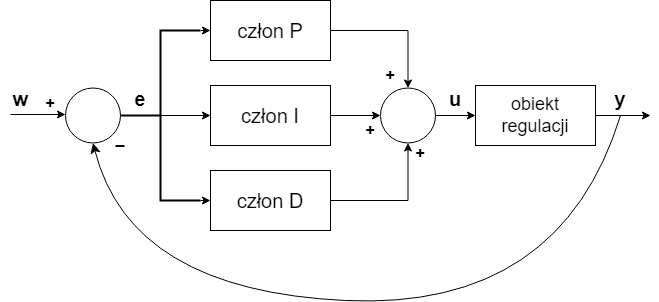
\includegraphics[width=0.8\textwidth]{./img/PID.png}
	\caption{Schemat blokowy regulatora PID}
	\label{fig:PID}
\end{figure}

\noindent Schemat z rys. 1.2 stanowi graficzną reprezentację matematycznej postaci regulatora PID.

\newpage
\subsubsection{Matematyczna postać regulatora PID \cite{knospe2006pid}}
\noindent Równanie czasowe regulatora:
\begin{equation}
	u(t)_{\text{PID}} = k_r \left( e(t) + \frac{1}{T_I} \int_{0}^{t} e(\tau) \, d\tau + T_D \frac{d(e(t))}{dt} \right)
\end{equation}

\noindent Opis oznaczeń:
\begin{description}
	\item[\textbf{u(t)$_\text{PID}$}:] sygnał sterujący w chwili $t$
	\item[\textbf{k$_r$}:] wzmocnienie proporcjonalne
	\item[\textbf{e(t)}:] uchyb w chwili $t$
	\item[\textbf{T$_I$}:] czas całkowania
	\item[\textbf{T$_D$}:] czas różniczkowania
\end{description}

\noindent W dziedzinie operatorowej, transmitancja regulatora PID przyjmuje postać:

\begin{equation}
	K(s)_{\text{PID}} = k_r\left(1 + \frac{1}{T_I S} + T_D S\right)
\end{equation}\\

\noindent Formuły 1.1 oraz 1.2 reprezentują postać idealną, w której człon różniczkujący jest szczególnie podatny na występowanie szumów pomiarowych. W układach rzeczywistych, człon różniczkujący wymaga dodatkowej filtracji, co reazliuje wprowadzenie parametru $\alpha$ do równania. Równanie rzeczywistego regulatora PID przyjmuje wówczas postać:

\begin{equation}
	K(s)_{\text{PID}} = k_r\left(1 + \frac{1}{T_I s} + \frac{T_D s}{1 + \alpha T_D s}\right)
\end{equation}

\newpage
\subsubsection{Znaczenie odpowiedniej regulacji układu}
Wprowadzenie regulacji PID pozwala na określenie zależności pomiędzy parametrami, wpływającymi na procesy zachodzące w układzie. Dodatkowo, cały proces odbywa się w sposób ciągły, bez konieczności ingerencji operatora. W wielu przypadkach, już sama ciągła optymalizacja zmienności kluczowych parametrów, może przełożyć się na działanie elementów wykonawczych i w efekcie spowodować znaczące zmniejszenie ich zużycia. W rozważanym układzie cieplnym, regulator PID odpowiada za dobór odpowiedniej mocy pieca, w zależności od temperatury zadanej i temperatury wylotowej. Uwzględnienie w regulacji wszystkich trzech członów (P, I, D) pozwoli odpowiednio reagować zarówno na nagłe zmiany, takie jak zmiana temperatury wlotowej (człon P), zmniany w kontekście dłuższego czasu pracy (człon I), czy bezwładność cieplną układu (człon D). Zagadnienie regulacji jest niezwykle istotne, jednak w kontekście przedstawionego problemu, sama regulacja nie przekłada się, w sposób bezpośredni, na zużycie przekaźników zasilających grzałki. Znacznie większy wpływ powinno mieć zastosowanie przemyślanego algorytmu, sterującego urządzeniem wykonawczym. Powody takiego stanu rzeczy zostaną wytłumaczone w następnym rozdziale. Nie oznacza to jednak, że sama regulacja jest bez znaczenia, bowiem algorytm zmniejszający zużycie przekaźników będzie korzystał z optymalnych parametrów, uzyskanych dzięki procesowi regulacji.

\subsection{Zdefiniowanie celu pracy}
Tematem pracy jest implementacja, optymalizacja oraz analiza działania różnych wersji algorytmu, sterującego urządzeniem wykonawczym, w kontekście rzeczywistego układu regulacji. Algorytmy są dedykowane dla instalacji cieplnej, której najważniejszy element stanowi elektryczny piec przepływowy, wyposażony w trzy grzałki zasilane jednofazowo. Głównym celem optymalizacji algorytmu jest minimalizacja liczby przełączeń przekaźników, zasilających grzałki pieca, przy zachowaniu równomiernego obciążenia poszczególnych grzałek.

\chapter{Charakterystyka elementów wykonawczych}
\label{ch:02}
\subsubsection{Podział ze względu na wykorzystane zjawiska fizyczne}
Elementy wykonawcze można sklasyfikować ze względu na rodzaj wielkości fizycznej, wykorzystywanej do wytworzenia siły, potrzebnej do oddziaływania na obiekt. Charakterystyka dzieli urządzenia na takie jak: pneumatyczne, hydrauliczne, termiczne, magnetyczne, elektromagnetyczne, elektrostatyczne, elektromechaniczne, czy piezoelektryczne. Przekaźniki zaliczają się do elementów elektromagnetycznych, których funkcja polega na przełączaniu określonych elementów obwodu elektrycznego. W instalacji cieplnej wykorzystano przekaźniki SSR, które kontrolują przepływ prądu, poprzez wykorzystanie elementów półprzewodnikowych (tranzystory, triaki), zamiast tradycyjnych elementów mechanicznych (cewka, styki). Przekaźniki są sterowane napięciem 24 V DC, z maksymalnym obciążeniem prądowym, wynoszącym 20 A. Brak elementów mechanicznych zapewnia cichszą pracę, szybsze przełączanie oraz poprawę bezpieczeństwa, ze względu na wyeliminowanie ryzyka powstawania łuków elektrycznych. W instalacji tego typu możliwe byłoby również zastosowanie styczników, jednak nie byłoby możliwe sterowanie każdą fazą z osobna, gdyż styczniki są zazwyczaj elementami trójfazowymi. Grzałki przemysłowe to elementy termiczne, zasilane za pomocą trzech faz wszędzie tam, gdzie konieczne jest wykorzystywanie dużych mocy. Mniejsze urządzenia wyposażone są w grzałki jednofazowe.

\begin{figure}[h]
	\centering
	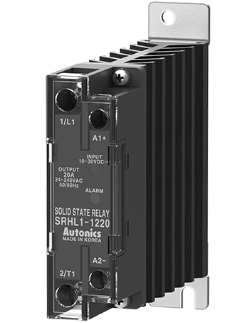
\includegraphics[width=0.19\textwidth]{./img/SSR2.png}
	\caption{Przekaźnik SRHL1-1220 wykorzystany w instalacji \cite{autonics}}
	\label{fig:SSR}
\end{figure}

\newpage
\subsubsection{Podział ze względu na rodzaj sygnału}
W kontekście opisywanego tematu, za bardziej istostny należy jednak uznać podział ze względu na rodzaj sygnału steruącego. Najczęściej spotykane są układy analogowe, reprezentowane w formie ciągłych wartości, w postaci napięcia lub natężenia prądu, które powodują stopniową zmianę sygnału sterującego (np. praca zaworu). Drugim rodzajem są elementy dwustanowe (cyfrowe). Układy cyfrowe pozwalają na uzyskanie dyskretnej reprezentacji sygnałów. To oznacza, że sygnały przyjmują skończoną liczbę możliwych wartości, natomiast sygnały analogowe mogą przyjmować nieskończenie wiele wartości, w danym zakresie, przez co są bardzo precyzyjne. Nie wymagają również procesu kwantyzacji i są bardziej elastyczne, jeśli chodzi o szybkość zmian wartości. Ze względu na większą zgodność z fizyczną naturą zjawisk (płynnosć, nieprzerwalność), sygnały analogowe często są bardziej naturalnym wyborem, podczas konstruowania układów automatyki. Implementowanie sterowania ciągłego wymaga jednak stosowania urządzeń elektroniki analogowej, co zazwyczaj zwiększa zarówno koszta, jak i skomplikowanie struktury układu. Ze względu na to, że sterowanie cyfrowe cechuje znacznie większa prostota implementacji, wykorzystuje się je wszędzie tam, gdzie takie rozwiązanie jest wystarczarczające, czyli w urządzeniach o stosunkowo prostej strukturze. Przykładem takiego urządzenia jest właśnie grzałka.

\begin{figure}[h]
	\centering
	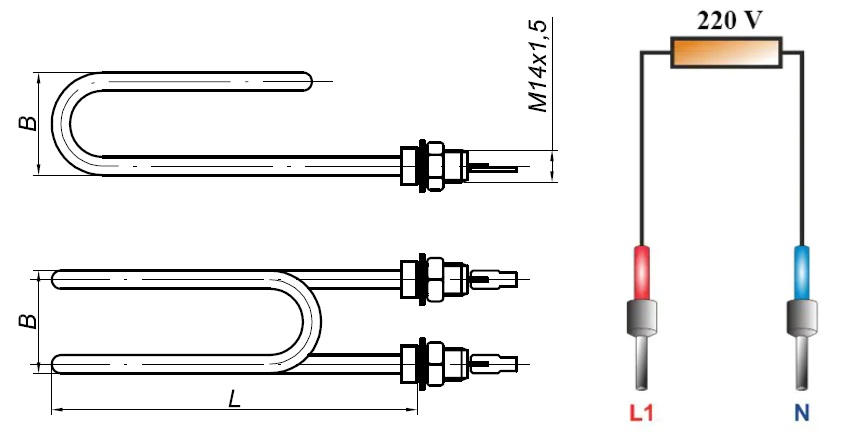
\includegraphics[width=0.6\textwidth]{./img/onePhaseHeater.jpg}
	\caption{Zasilanie grzałki jednofazowej \cite{egniazdka, intmax}}
	\label{fig:onePhaseHeater}
\end{figure}

\begin{figure}[h]
	\centering
	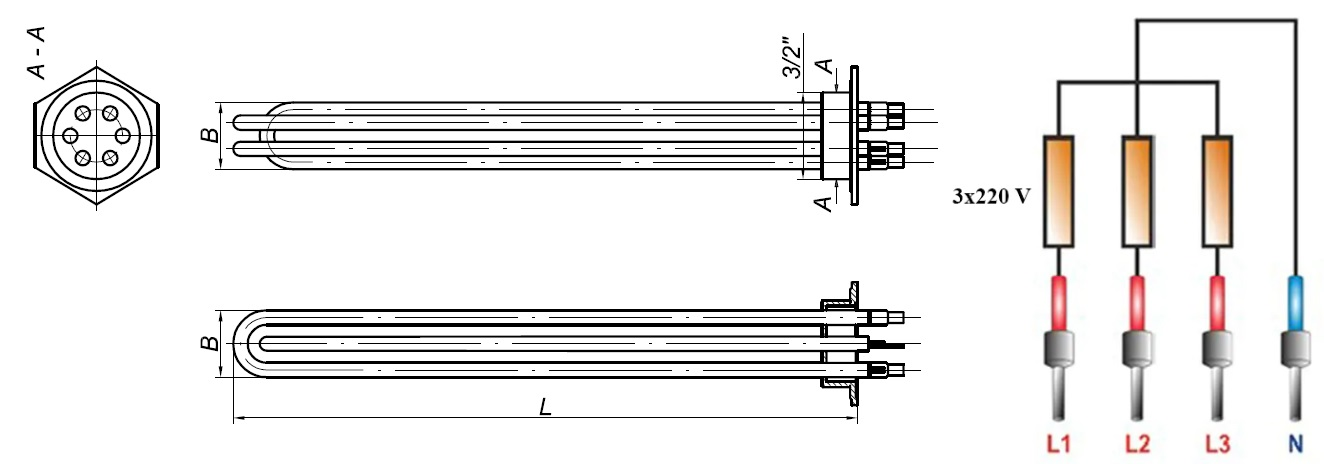
\includegraphics[width=0.8\textwidth]{./img/threePhaseHeater.jpg}
	\caption{Zasilanie grzałki trófazowej (gwiazda) \cite{egniazdka, intmax}}
	\label{fig:threePhaseHeater}
\end{figure}

\chapter{Założenia projektowe}
\label{ch:03}
Aby osiągać pożądane wartości tempeartury cieczy, należy określać chwilową moc efektywną pieca, w precyzyjny sposób (przykładowo z dokładnością do 1\%). Tę wartość należy następnie odnieść do efektywnej mocy grzałek, również z przedziału procentowego <0, 100>. Dokładne przełożenie tych wartości na fizyczny model, w dowolnej chwili czasu, byłoby możliwe jedynie poprzez uzyskiwanie pomiarów w sposób ciągły. Sygnał sterujący przekaźnikiem przyjmuje jednak wartość 0 lub 1, co przekłada się na 0\% lub 100\% mocy grzałki. Należy więc znaleźć rozwiązanie, które pozwoli na włączanie i wyłączanie grzałek w taki sposób, aby suma średnich wartości ich mocy, w określonym przedziale czasowym, miała wystarczająco dokładne przełożenie na wysterowywaną moc pieca. Innymi słowy, przełączanie grzałek w odpowiednich cyklach ma służyć uzyskiwaniu pewnego rodzaju pseudociągłych charakterystyk mocy grzałek. Grzałki charakteryzują się zdolnością do szybkiego osiągnięcia zadanej temperatury i utrzymywania jej przez określony czas, w związku z czym, odpowiednie podejście do sterowania cyfrowego pozwoli skuteczenie zapanować nad układem.

\subsection{Metoda modulacji sygnału}
Do uzyskania pożądanej mocy średniej w czasie, zastosowany zostanie powszechnie znany sposób modulacji - modulacja szerokości impulsów PWM (ang. pulse-width modulation) \cite{sun2012pulse}. PWM pozwala na regulację mocy dostarczanej do urządzenia, poprzez definiowanie czasu trwania sygnału impulsowego, załączającego urządzenie. Sygnał PWM składa się z dwóch podstawowych parametrów: okresu i współczynnika wypełnienia. Okres to czas cykliczego powtórzenia sygnału, a współczynnik wypełnienia to procent okresu, w którym sygnał znajduje się w stanie wysokim (włączony).

\begin{figure}[h]
	\centering
	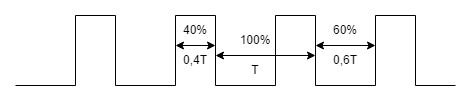
\includegraphics[width=0.8\textwidth]{./img/PWM.png}
	\caption{Sygnał PWM o współczynniku wypełnienia 40\% (T - okres PWM)}
	\label{fig:PWM}
\end{figure}

\noindent Współczynnik wypełnienia reprezentuje efektywny procent mocy grzałki. Algorytm pozwoli na odpowiedni dobór współczynnika każdej z grzałek, więc będą one pobudzane szeregiem takich impulsów. Można zauważyć, że długość okresu jest odwrotnie proporcjonalna do liczby przełączeń, którą algorytm powinien minimalizować.

\newpage
\noindent Warto jednak pamiętać o tym, że wybór zbyt długiego okresu PWM może skutować niepożądanymi wahaniami temperatury, gdyż piec jest obiektem charakteryzującym się sporą bezwładnością cieplną. Dynamika obiektu jest więc istotnym czynnikiem podczas doboru okresu PWM.

\subsection{Zdefiniowanie celów algorytmu}
Praca ma na celu porównanie dwóch podejść do sterowania układem. Pierwszy model sterowania piecem zakłada klasyczne sterowanie w trybie jednofazowym, gdzie wszystkie trzy grzałki sterowane sa za pomocą tego samego sygnału PWM. To oznacza, że w dowolnej chwili czasu, wszystkie grzałki znajdują się w tym samym stanie (0 lub 1). Pozwala to na równomierne rozłożenie pracy pomiędzy grzałkami, pod kątem dystrybucji ciepła oraz liczby przełączeń na stykach, w dowolnie krótkim przedziale czasowym.\\

Suma czasów stanu wysokiego i niskiego, stanowi czas pracy pojedynczego cyklu przełączenia grzałki (okres PWM). Warto zwrócić uwagę na pracę przekaźników, które w ciągu jednego takiego cyklu, za każdym razem zostają przłączone dwukrotnie (włączenie i wyłączenie), niezależnie od zadanego obciążenia (wypełnienia PWM). Piec to urządzenie pracujące zazwyczaj przez dłuższy czas, a przełączanie przekaźników jest bardzo częste. Sumaryczna liczba przełączeń jest więc ogromna i powoduje szybkie zużycie elementów wykonawczych. Prostym sposobem na zmniejszenie tych obciążeń, w modelu jednofazowym, jest maksymalne zwiększenie okresu PWM w taki sposób, aby temperatura pieca nie ulegała zbyt wysokim wahaniom. Rozwiązanie takie nie jest jednak uniwersalne, ponieważ zależy od właściwości dynamicznych konkretnej instalacji cieplnej, takich jak bezwładność termiczna, charakterystyka izolacji, zdolność regulacyjna, rozmiar pieca itp.

\newpage
Biorąc pod uwagę fakt, że w układzie każda grzałka zasilana jest z innej fazy, można szybko dojsć do wniosku, że sterowanie synchroniczne znacząco ogranicza możliwości optymalizacyjne. Nasuwa się wniosek, że możliwe jest stworzenie usprawnionego algorytmu sterowania, który dla dowolnej ustalonej wartości mocy pieca, lepiej poradzi sobie z zagadnieniem częstości przełączania styków, poprzez chwilowe nierównomierne obciążanie grzałek. Zmiana tych obciążeń w czasie, powinna jednak umożliwić uzyskanie zbliżonej liczby przełączeń przekaźników, w perpektywie dłuższego czasu pracy instalacji. Jednocześnie należy pamiętać, że dla określonej instalacji (konkretnego pieca i układu regulacji), usprawniony algorytm powinien utrzymywać temperaturę oraz jej wahania na bardzo podobnym poziomie, jak w przypadku zastosowania koncepcji jednofazowej, a także umożliwić precyzyjny dobór mocy pieca. Na podstawie mocy pieca, do poszczególnych faz przydzielone zostaną współczynniki wypełnienia PWM. Regulacja mocy pieca zostanie uzależniona od temperatury zadanej, na wyjściu z instalacji. Ponadto, działanie algorytmu powinno być przewidywalne i uniwersalne, aby nie utrudniać samego procesu regulacji.\\

\subsection{Optymalizacja w odniesieniu do układu regulacji}
W ramach pracy rozważany jest układ cieplny z obiektem regulacji, w postaci elektrycznego pieca przepływowego, służącego do podgrzewania cieczy. Piec wyposażony został w elementy wykonawcze, w postaci zaworów oraz trzech grzałek, zasilanych za pomocą przekaźników. Układ składa się również z wielu elementów pomiarowych, takich jak przepływomierze elektromagnetyczne, czujniki ciśnienia, czy przetworniki temperatury. Rozważana w ramach pracy optymalizacja algorytmu, skupia się jednak wyłącznie wokół sposobu sterowania grzałkami, w zależności od parametru mocy zadanej. Wobec tego, zdefiniowany układ regulacji będzie realizował ustalanie mocy pieca (wartość sterowana), na podstawie temperatury zadanej (wartość zadana) oraz temperatury wylotowej (wartość regulowana). Moc pieca zostanie przełożona, w sposób bezpośredni, na wypełnienie sygnałów PWM poszczególnych grzałek.\\

Podsumowując, celem pracy jest stworzenie uniwersalnego algorytmu, sterującego trzema fazami pieca niezależnie, który ostatecznie pozwoli na równomierne zmniejszenie liczby przełączeń przekaźników. Takie podejście zostało umożliwione, dzięki obecności w instalacji trzech grzałek, sterowanych za pomocą osobnych przekaźników.

\newpage
\subsection{Poglądowe schematy instalacji}
\begin{figure}[h]
	\centering
	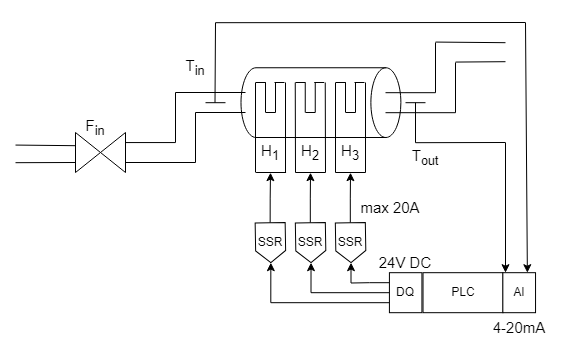
\includegraphics[width=0.75\textwidth]{./img/system.png}
	\caption{Schemat instalacji}
	\label{fig:System}
\end{figure}

\begin{figure}[h]
	\centering
	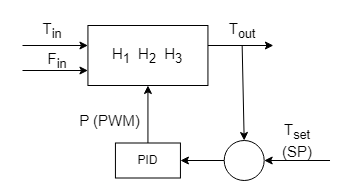
\includegraphics[width=0.55\textwidth]{./img/systemRegulation.png}
	\caption{Schemat instalacji w ujęciu sposobu regulacji}
	\label{fig:System regulation}
\end{figure}

\noindent Opis oznaczeń:
\begin{description}
	\item[\textbf{F$_{\text{in}}$}:] przepływ wlotowy
	\item[\textbf{T$_{\text{in}}$}:] temperatura wlotowa cieczy
	\item[\textbf{T$_{\text{out}}$}:] temperatura wylotowa cieczy
	\item[\textbf{T$_{\text{set}}$}:] temperatura zadana
	\item[\textbf{P(PWM)}:] moc pieca (od której zależy wypełnienie PWM)
	\item[\textbf{H$_{\text{1}}$, H$_{\text{2}}$, H$_{\text{3}}$}:] oznaczenia grzałek
	\item[\textbf{AI}:] wejścia analogowe
	\item[\textbf{DQ}:] wyjścia cyfrowe
\end{description}

% TODO
\chapter{Wymagania i narzędzia}
\label{ch:04}

Rozdział skupia się wyłącznie na procesie tworzenia struktury oraz logiki algorytmu, wraz z wynikami symulacji działania, bez uwzględnienia implementacji na rzeczywistym układzie regulacji.

\subsection{Wykorzystane narzędzia}
Program napisano z myślą o sterowniku z seri S7-1500, wyprodukowanym przez znany niemiecki koncern Siemens, konkretnie modelu \textbf{1516-3 PN/DP}, podłączonego do instalacji cieplnej. Realizację projektu umożliwił szereg narzędzi dostarczonych przez tego samego prodeucenta, wraz z oprogramowaniem \textbf{TIA Portal (V17)}\cite{berger2013automating}. Symulację algorytmu przeprowadzono przy pomocy dodatkowego oprogramowania \textbf{S7-PLCSIM (V17)}. Narzędzie pozwala zasymulować działanie tworzonego programu, na dowolnym sterowniku firmy Siemens. Do wizualizacji wyników wykorzystano środowisko \textbf{Matlab}.

\subsection{Struktura programu}
Funkcję, realizującą główne cele algorytmu, opisano w bloku \textit{ExecutePWM}. Blok opisuje logikę obejmującą wszystkie główne założenia projektowe, synchronizację kroków, wprowadzone zabezpieczenia itp. Wewnątrz bloku \textit{ExecutePWM} zagnieżdżono blok \textit{CalculatePWM}, który odpowiada wyłącznie za proces generowania sygnału PWM i tym samym zmianę stanu każdej z grzałek. Oprócz tego, stworzono funkcję o nazwie \textit{Analysis}, która nie jest bezpośrednio związana z działaniem algorytmu i służy jedynie do automatycznego generowania przykładowych przypadków pomiarowych oraz zbierania danych, potrzebnych do późniejszej analizy skuteczności.

\newpage
\subsubsection{Funkcja \textit{ExecutePWM}}
Dane wejściowe oraz wyjściowe funkcji głównej \textit{ExecutePWM} można odczytać z rysunku zamieszczonego poniżej.

\begin{figure}[h]
	\centering
	\includegraphics[width=0.8\textwidth]{./img/ExecutePWM.png}
	\caption{Blok funkcji \textit{ExecutePWM}}
	\label{fig:ExecutePWM}
\end{figure}

Jako wejście funkcja przyjmuje: moc pieca \textit{I\_furnancePower (Real, \%)}, okres PWM \textit{I\_cycleTime (Real, s)} oraz zmienne określające wybrany tryb pracy - jednofazowy lub trójfazowy \textit{IO\_one/threePhaseSwitch (Bool)}. Na wyjściu funkcja zwraca aktualną wartość stanu (wysoki, niski) poszczególnych grzałek, przekazywaną bezpośrednio na adresy wyjściowe sterownika, odpowiadające za ich włączanie oraz wyłączanie.

\subsubsection{Wyznaczanie współczynnika \textit{heaterFactor}}
Na początku należy obliczyć parametry, które stanowią fundament poprawnego działania pozostałej części algorytmu. Pierwszym krokiem będzie obliczenie współczynnika o nazwie \textit{heaterFactor (Real)}. Piec składa się z trzech grzałek, więc można założyć, że każdy 1\% mocy pieca przekłada się na 3\% mocy pojedynczej grzałki (100\% mocy każdej grzałki przekłada się na 33,(3)\% mocy pieca). Wartość współczynnika mieści się więc w przedziale <0, 300> i odpowiada sumie procentowej obciążenia wszystkich grzałek. Współczynnik stanowi wartość wyjściową, która w kolejnych krokach umożliwi obliczenie poszczególnych wypełnień PWM.

\newpage
\subsubsection{Przydzielenie obciążeń}
Teraz można przydzielić wypełnienia PWM grzałek, dla trybu trójfazowego, na podstawie współczynnika \textit{heaterFactor}. Do kolejnych zmiennych pomocniczych przydzielane są maksymalne możliwe wartości procentowe wypełnienia \textit{first/second/thirdFilling (Real, \%)}, zgodnie ze wzorem:

\[ f_j = h_f - 100(j - 1)\]
\noindent Gdzie:\\
$h_f$: \textit{heaterFactor} $\in$ <0, 300>\\
$f_j$: procent wypełnienia grzałki nr j $\in$ <0, 100>\\
$j$: iteracja przypisania $\in$ \{1, 2, 3\}\\

\noindent Obliczone w ten sposób wartości zostają przypisane do zmiennych pomocniczych. Wartości zmiennych zostaną przydzielone do odpowiednich grzałek natychmiast, gdy tylko program wykryje uruchomienie trybu trójfazowego. Jeżeli aktywowano tryb jednofazowy, do zmiennych pomocniczych przypisany zostanie identyczny współczynnik wypełnienia, zgodny z procentową wartością mocy użytkowej pieca, w aktualnej chwili czasu. Ostatnim krokiem bloku \textit{ExecutePWM} jest podanie obliczonych współczynników wypełnienia, na wejścia bloku funkcji \textit{ControlPWM}, widocznego na rysunku 4.2.\\

\subsubsection{Zastosowanie funkcji ControlPWM}
Niektóre modele sterowników Siemensa (przykładowo 1212C DC/DC/DC) z wyjściami tranzystorowymi, umożliwiają skonfigurowanie wyjść cyfrowych w TIA Portal, jako wyjścia impulsowe (PTO lub PWM), a następnie konfigurację sygnału, za pomocą dostarczonej funkcji \textit{CTRL\_PWM}. Model sterownika, obecnego w instalacji, nie oferuje jednak konfiguracji pozwalającej na użycie funkcji \textit{CTRL\_PWM}. Funkcja \textit{ControlPWM} wykonana w ramach tej pracy, ma na celu umożliwienie realizacji podobnego działania.

\newpage
\begin{figure}[h]
	\centering
	\includegraphics[width=0.8\textwidth]{./img/ControlPWM.png}
	\caption{Blok funkcji \textit{ControlPWM}}
	\label{fig:ControlPWM}
\end{figure}

Wspomniane zmienne pomocnicze \textit{first/second/thirdHeater} przechowują w sobie aktualizowane na bieżąco współczynniki wypełnienia (zależne od \textit{heaterFactor} i wybranego trybu pracy). Na ich postawie funkcja \textit{ControlPWM} zwraca aktualne stany sygnałów, które zostają przepisane bezpośrednio na fizyczne wyjścia cyfrowe, sterujące przekaźnikami. Sterowanie wypełnieniem zostało zrealizowane poprzez zastosowanie timerów \textit{TON}. Fragment kodu odpowiadającego za sterowanie pojedynczą grzałką, w trybie trójfazowym, zamieszczono poniżej.

\begin{figure}[h]
	\centering
	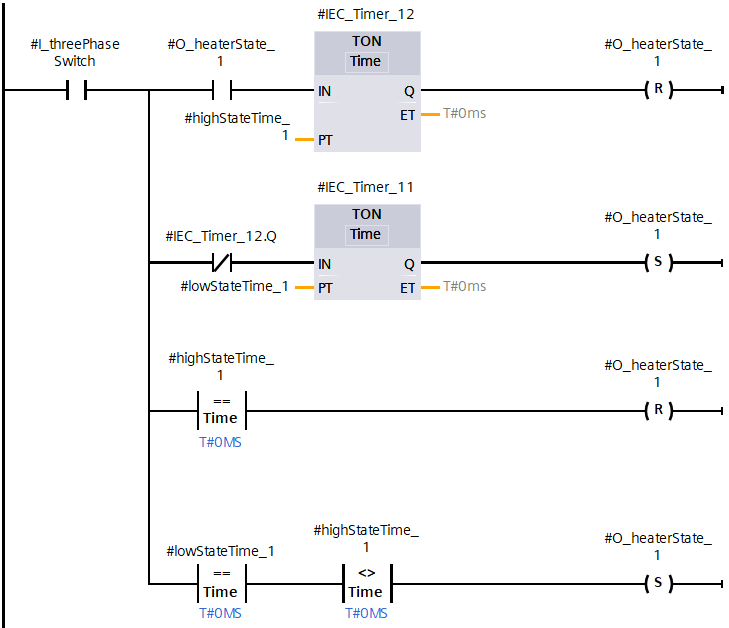
\includegraphics[width=0.78\textwidth]{./img/controlPWMcut.png}
	\caption{Kontrola wypełnienia PWM przy użyciu timerów \textit{TON}}
	\label{fig:ControlPWM cut}
\end{figure}

\newpage
\subsubsection{Wykorzystanie timera \textit{TON} w bloku \textit{ControlPWM}}
Zegar rozpoczyna odmierzanie czasu, gdy zmienna powiązana z parametrem wejściowym \textit{IN} zmieni stan z niskiego na wysoki (zobocze narastające). W tym momencie rozpoczyna się odmierzanie czasu opóźnienia \textit{PT}, po którym parametr wyjściowy \textit{Q} zmienia stan na wysoki. Stan wysoki parametru \textit{Q} zostaje utrzymany do momentu, w którym parametr \textit{IN} powraca do stanu niskiego (zbocze opadające).

\begin{figure}[h]
	\centering
	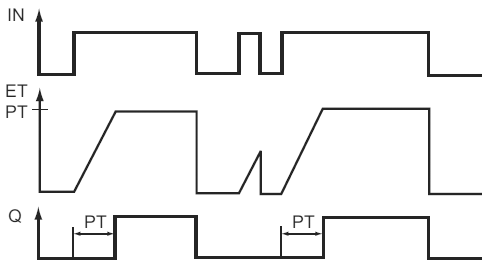
\includegraphics[width=0.7\textwidth]{./img/timerTON.png}
	\caption{Przykładowy przebieg czasowy timera \textit{TON} \cite{blogplc}}
	\label{fig:TON}
\end{figure}

Model opiera się na dwóch timerach \textit{TON} (timer on delay), oznaczonych na rysunku 4.3, jako \textit{IEC\_Timer\_12} (zegar A) i \textit{IEC\_Timer\_11} (zegar B). Jeżeli stan wyjściowy sygnału grzałki jest wysoki, uruchomiony zostaje timer A, który jako opóźnienie przyjmuje czas stanu wysokiego \textit{highStateTime\_X} (X - numer grzałki). Po tym czasie, wyjście \textit{Q} tego timera przyjmuje wartość 1, co z kolei zmienia stan sygnału grzałki na 0, za pomocą cewki resetującej. Zmiana stanu wyłącza działanie timera A, co powoduje jednocześnie uruchomienie timera B (oba timery nie mogą być aktywne jednocześnie). Opóźnienie aktywnego timera B odlicza w tej chwili czas, w którym grzałka powinna pozostać nieaktywna. Po tym czasie, stan sygnału ponownie zostaje zmieniony na wysoki i uruchomiony zostaje timer A (stanu wysokiego), a timer B wyłącza się. Następnie, cały cykl powtarza się wielokrotnie.
Powyższa logika nie działa prawidłowo, jeżeli któryś z czasów określających długość stanu jest zerowy. Zerowy czas stanu oznacza jednocześnie konieczność ciągłego podtrzymania stanu przeciwnego, co zostało uwzględnione, z odpowiednimi zabezpieczeniami, na dolnych gałęzaich kodu LAD (rys. 4.3).\\

Tryb jednofazowy opiera się na zasadzie działania analogicznej do trybu trójfazowego, z wyłączeniem zasady asynchronicznej pracy grzałek. Zmienne logiczne odpowiedzialne za stany grzałek, znajdują się teraz na jednej gałęzi programu (ten sam stan w dowolnym cyklu sterownika).

\newpage
\subsection{Symulacje sterowania układem}
Charakterystyczną cechą przedstawionego algorytmu optymalizacji jest to, że liczba aktywnych grzałek zmienia się w przedziałach co 33,(3)\% mocy użytkowej pieca (wielokrotność 1/3 mocy). Z tego powodu, wszystkie symulacje zostaną przeprowadzone dla wartości mocy użytkowej 20\%, 50\% i 80\% (po jednej wartości z każdego przedziału), co umożliwi efektywne zestawienie różnych podejść. Okres PWM ustalono na 1000 ms, a okres próbkowania co 10 ms. Każdy z przypadków będzie monitorowany przez 300 s, za pomocą narzędzia \textbf{Traces} dostępnego w środowisku TIA Portal. Narzędzie Traces służy do monitorowania i rejestrowania przebiegu programu sterującego, w czasie rzeczywistym. Dane zapisane do pliku CSV można następnie zwizualizować za pomocą środowiska Matlab. Liczba przełączeń przekaźników dla różnych przypadków, zostanie obliczona i zestawiona na końcu rozdziału.

\subsection{Sterowanie jednofazowe}
Dla wszystkich przykładów, liczba przełączeń przekaźników liczona jest dla czasu wynoszącego 300 s pracy układu. Liczba przełączeń stanowi sumę aktywacji i deaktywacji każdego przekaźnika. Przybliżenie odpowiednich fragmentów służy poprawie czytelności. Pełny przebieg czasowy zostanie zaprezentowany dla finalnej wersji algorytmu. Podawane wartości mocy są ideowe, wynikające wprost z zależności matemtycznych, wyłącznie na potrzeby symulacji.

\begin{figure}[h]
	\centering
	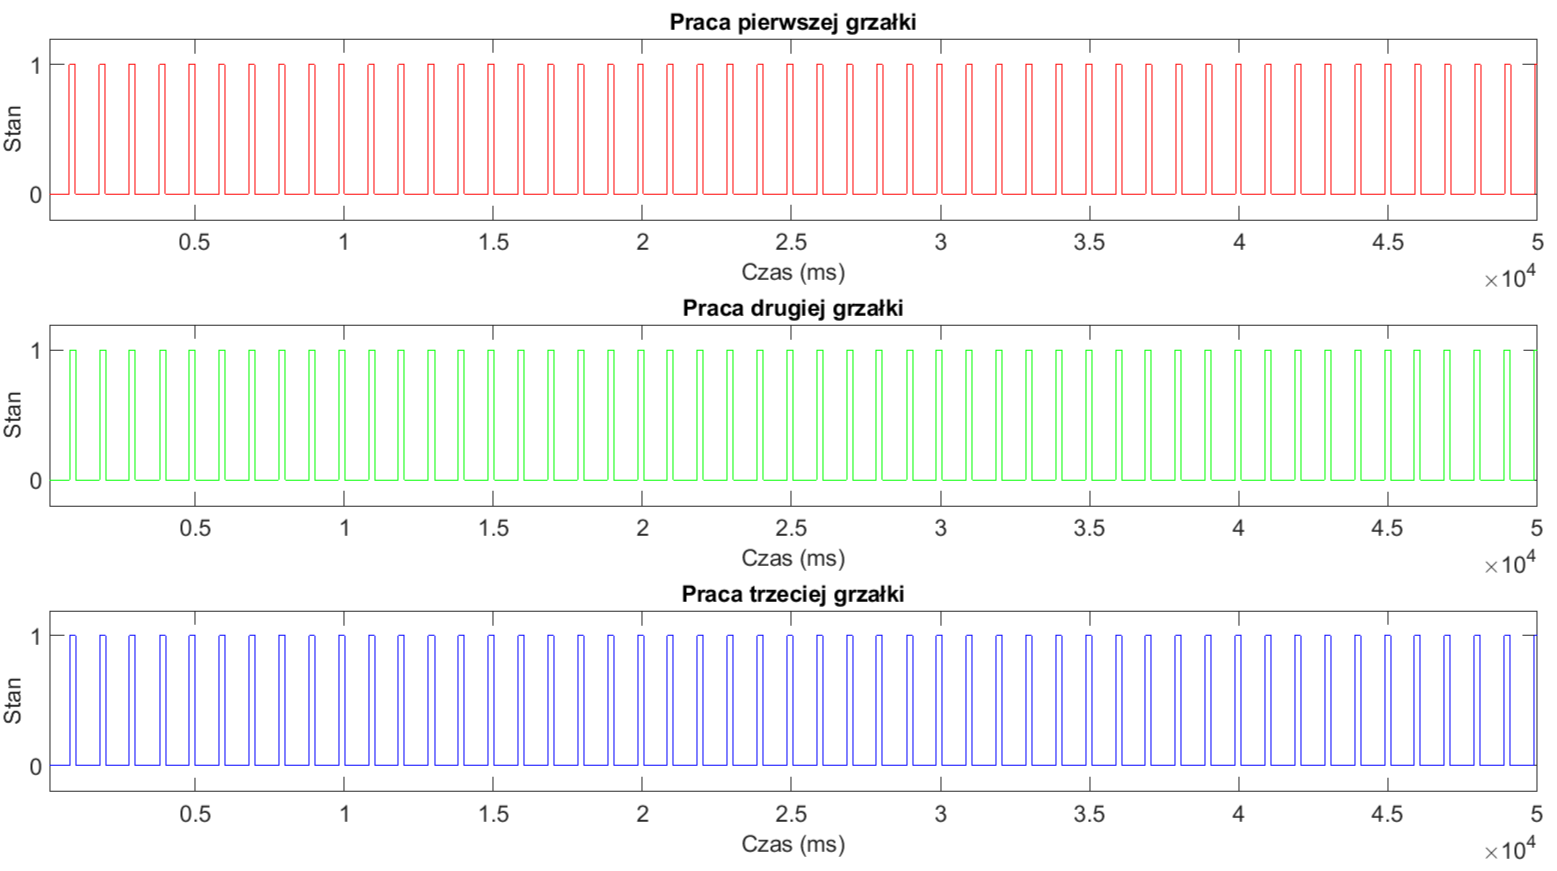
\includegraphics[width=0.94\textwidth]{./wykresy/png/onePhase20.png}
	\caption{Sterowanie jednofazowe (20\% mocy)}
	\label{fig:OnePhase20}
\end{figure}

\newpage
Z wykresów zamieszczonych powyżej można odczytać, że odpowiadające fragmenty przebiegów są ze sobą tożsame. Współczynnik wypełnienia jest identyczny dla każdej grzałki i odpowiada mocy użytkowej pieca 20\%, co jest zgodne z oczekiwaniami. Poniżej zamieszczono przebiegi dla 50\% i 80\% mocy użytkowej.

\begin{figure}[h]
	\centering
	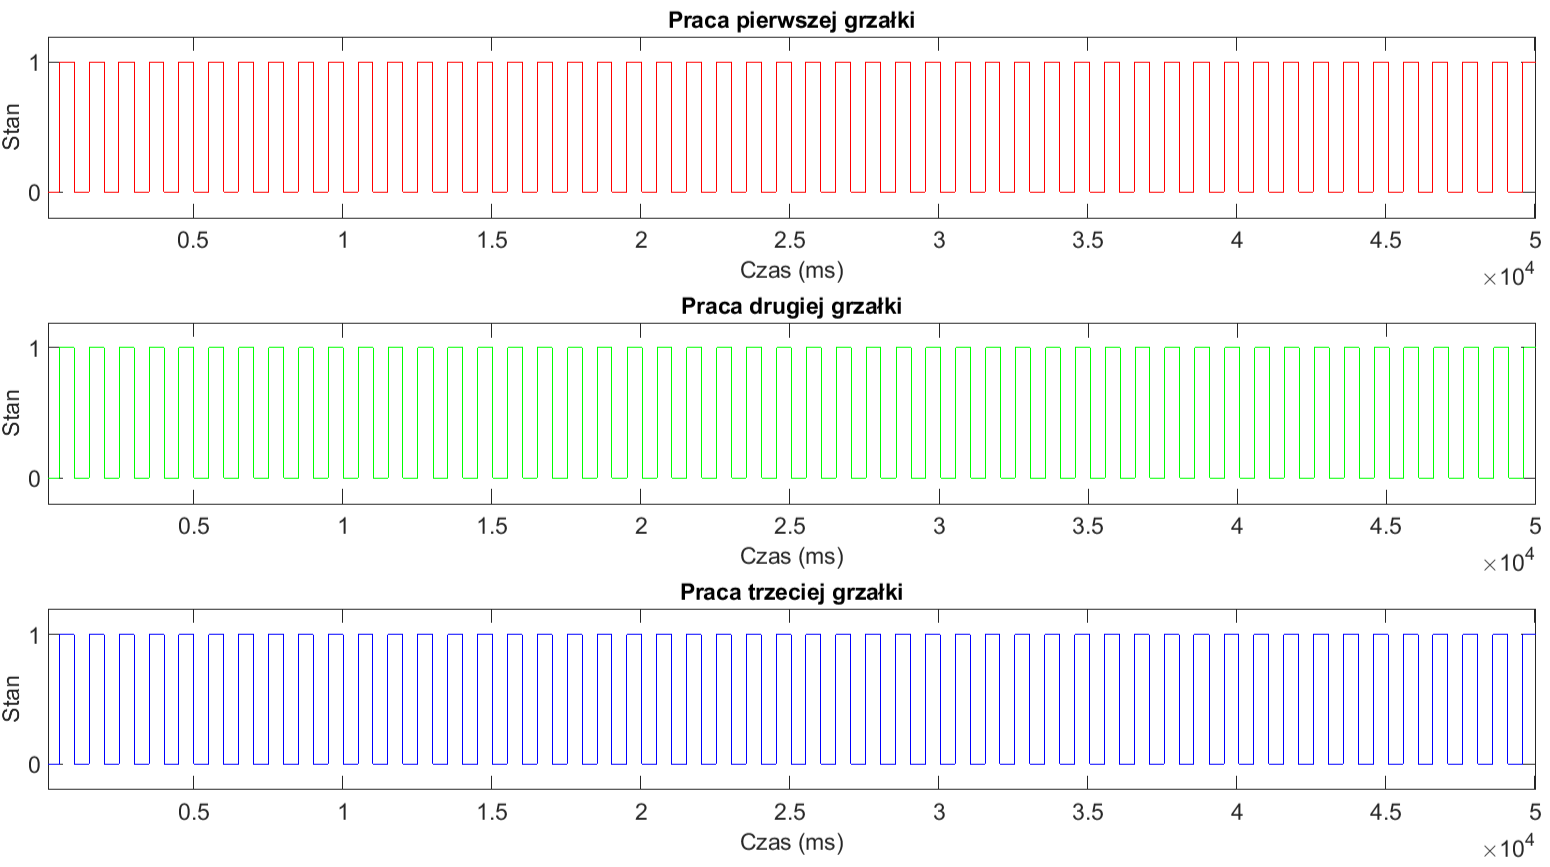
\includegraphics[width=0.92\textwidth]{./wykresy/png/onePhase50.png}
	\caption{Sterowanie jednofazowe (50\% mocy)}
	\label{fig:OnePhase50}
\end{figure}

\begin{figure}[h]
	\centering
	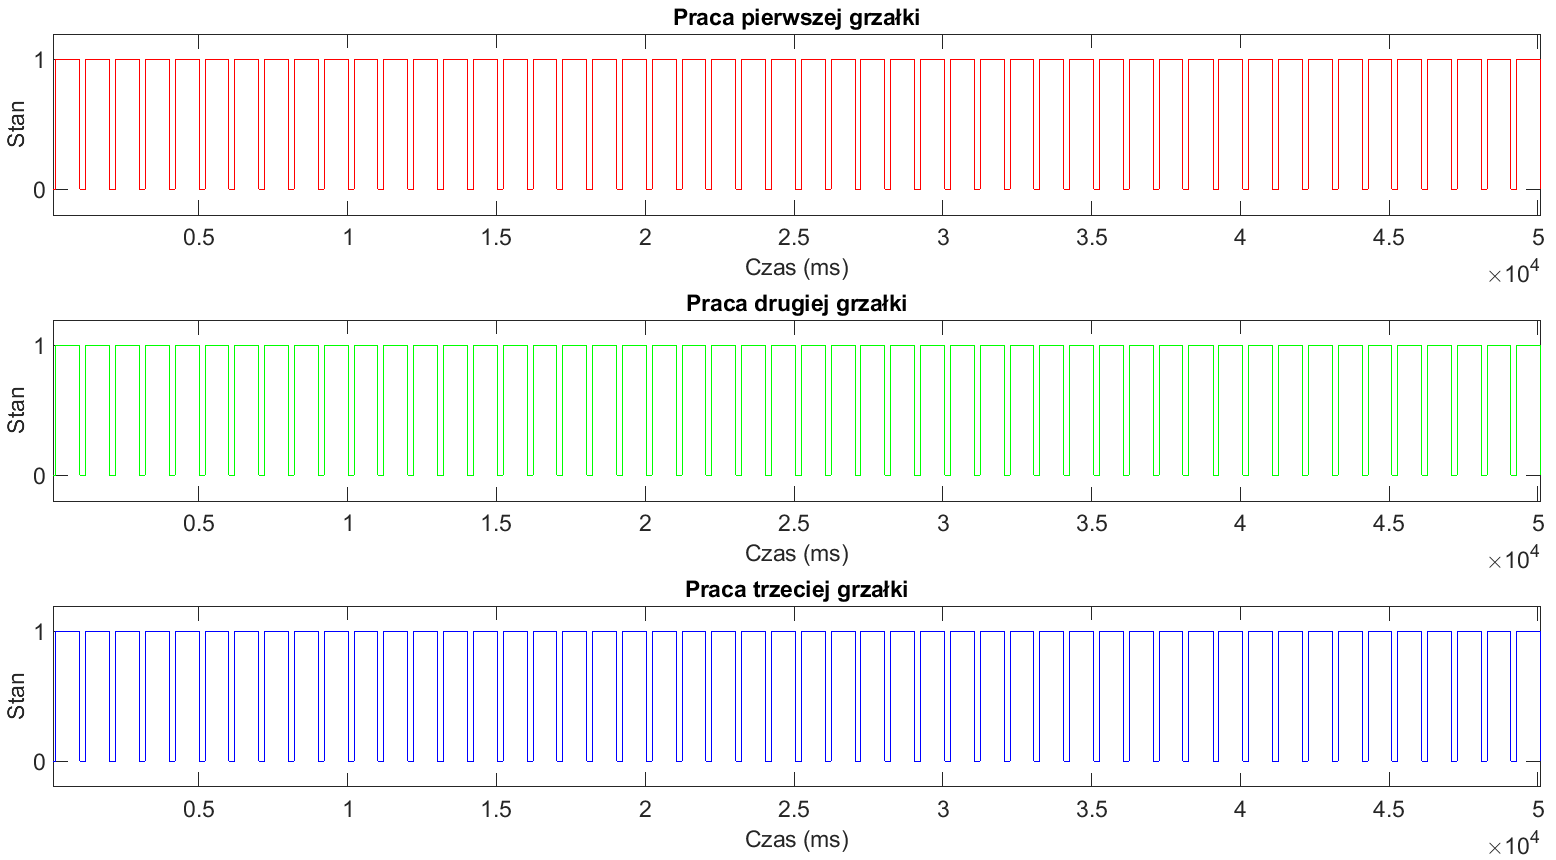
\includegraphics[width=0.92\textwidth]{./wykresy/png/onePhase80.png}
	\caption{Sterowanie jednofazowe (80\% mocy)}
	\label{fig:OnePhase80}
\end{figure}

\noindent Ogólna zasada działania sterowania jednofazowego nie ulega zmianie, niezależnie od aktualnej mocy użytkowej pieca. Dla wszystkich obciążeń liczba przełączęń przekaźników każdej z grzałek wyniosła po 598 lub 599 przełączeń (dokładne liczby w podsumowaniu).

\newpage
\subsubsection{Komentarz}
Sterując przełączeniami przkaźników jednofazowo, uzyskano równą liczbę przełączeń, niezależnie od zmiany wypełnienia PWM. Wynika to z faktu, że na liczbę przełączeń wpływa wyłącznie okres sygnału PWM. Jeżeli \(\text{moc pieca} \notin \{0, 100\}\), na każdy okres przypadają dokładnie dwa przełączenia. Kolejnym krokiem będzie więc nadanie nierównomiernego obciążenia w taki sposób, aby przypisywać każdej kolejnej grzałce maksymalne możliwe obciążenie. Wynik eksperymentu przedstawiono w kolejnej podsekcji.

\subsection{Realizacja nierównomiernego obciążenia grzałek}
\begin{figure}[h]
	\centering
	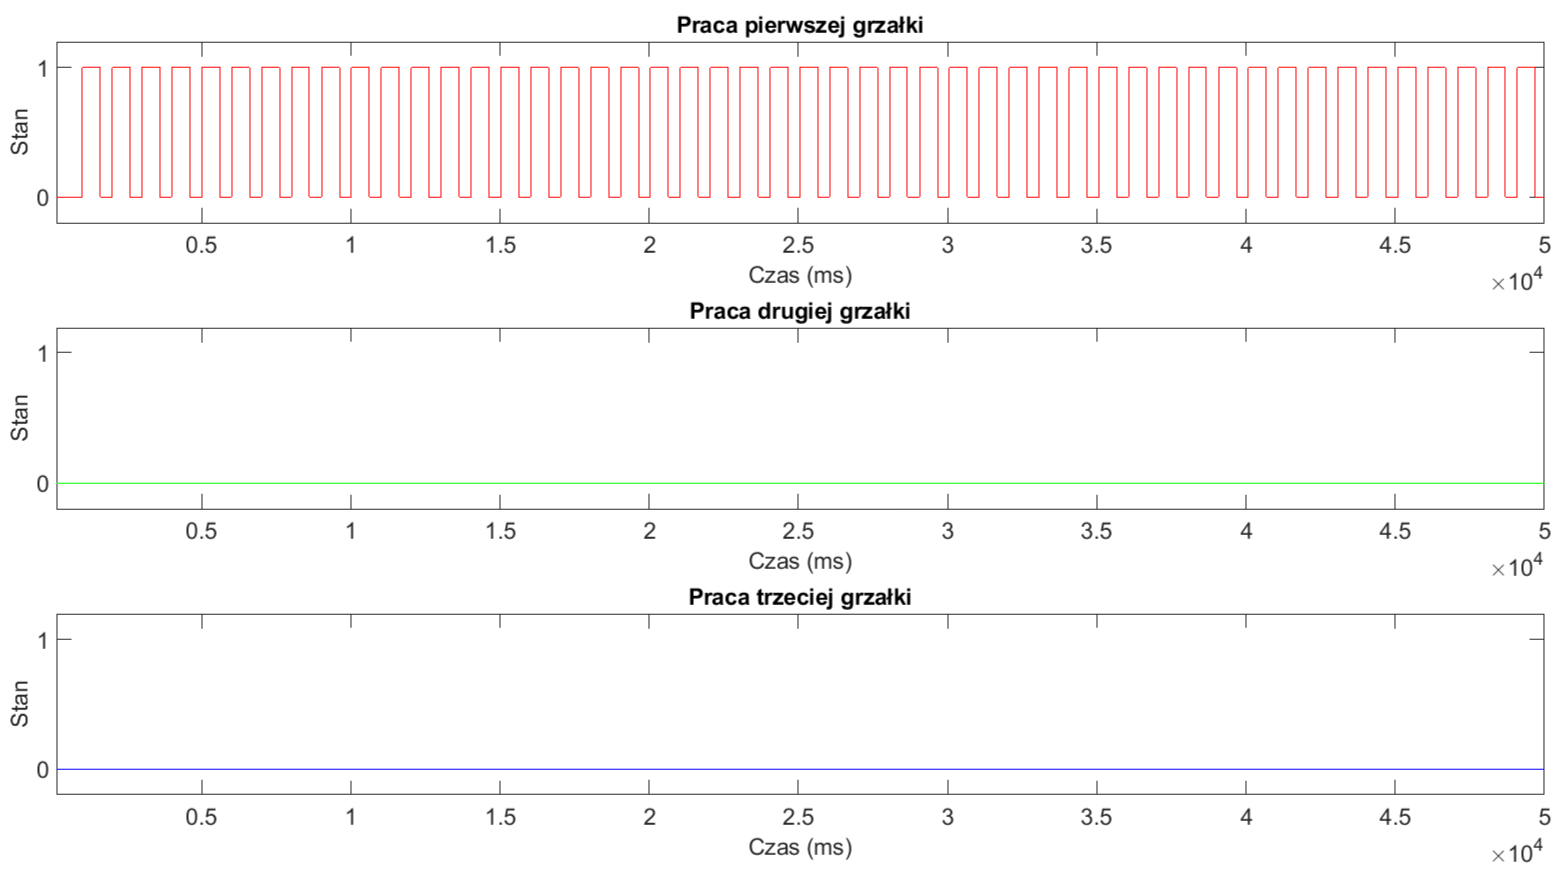
\includegraphics[width=0.92\textwidth]{./wykresy/png/threePhase20worse.png}
	\caption{Sterowanie trójfazowe (20\% mocy)}
	\label{fig:ThreePhase20worse}
\end{figure}

W tym przypadku grzałka pierwsza pierwsza (czerwona) działa z wypełnieniem 60\%, co stanowi trzykrotność zadanej mocy pieca. Wartość wynika z tego, że dwie pozostałe grzałki pozostają nieaktywne, więc praca grzałki trzeciej stanowi całkowitą wartość energii, wytwarzanej w układzie. Liczba przełączeń aktywnego przekaźnika wyniosła 599.

\newpage
\begin{figure}[h]
	\centering
	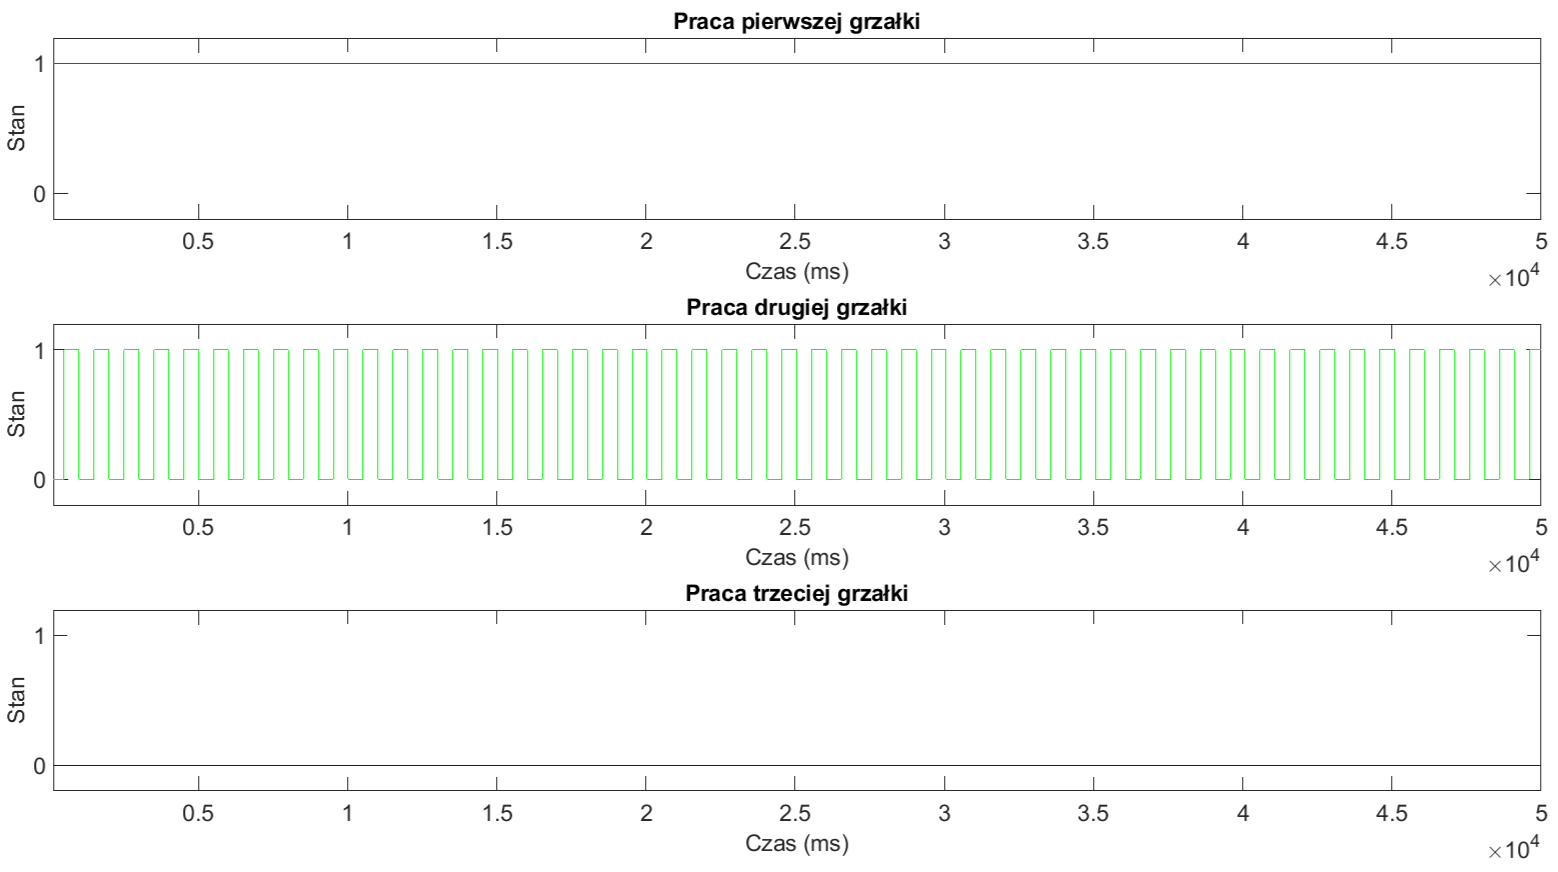
\includegraphics[width=0.92\textwidth]{./wykresy/png/threePhase50worse.png}
	\caption{Sterowanie trójfazowe (50\% mocy)}
	\label{fig:ThreePhase50worse}
\end{figure}

\noindent Pierwsza grzałka została przełączona w stały tryb pracy, więc wytwarza 33,(3)\% całkowitej mocy pieca, a liczba przełączeń przekaźnika wyniosła 1 (włączenie). Grzałka trzecia (niebieska) pozostaje nieaktywna. Grzałka druga wytwarza pozostałą część energii (17\%), co przekłada się na współczynnik wypełnienia równy 51\%. Liczba przełączeń przekaźnika wyniosła 600.

\begin{figure}[h]
	\centering
	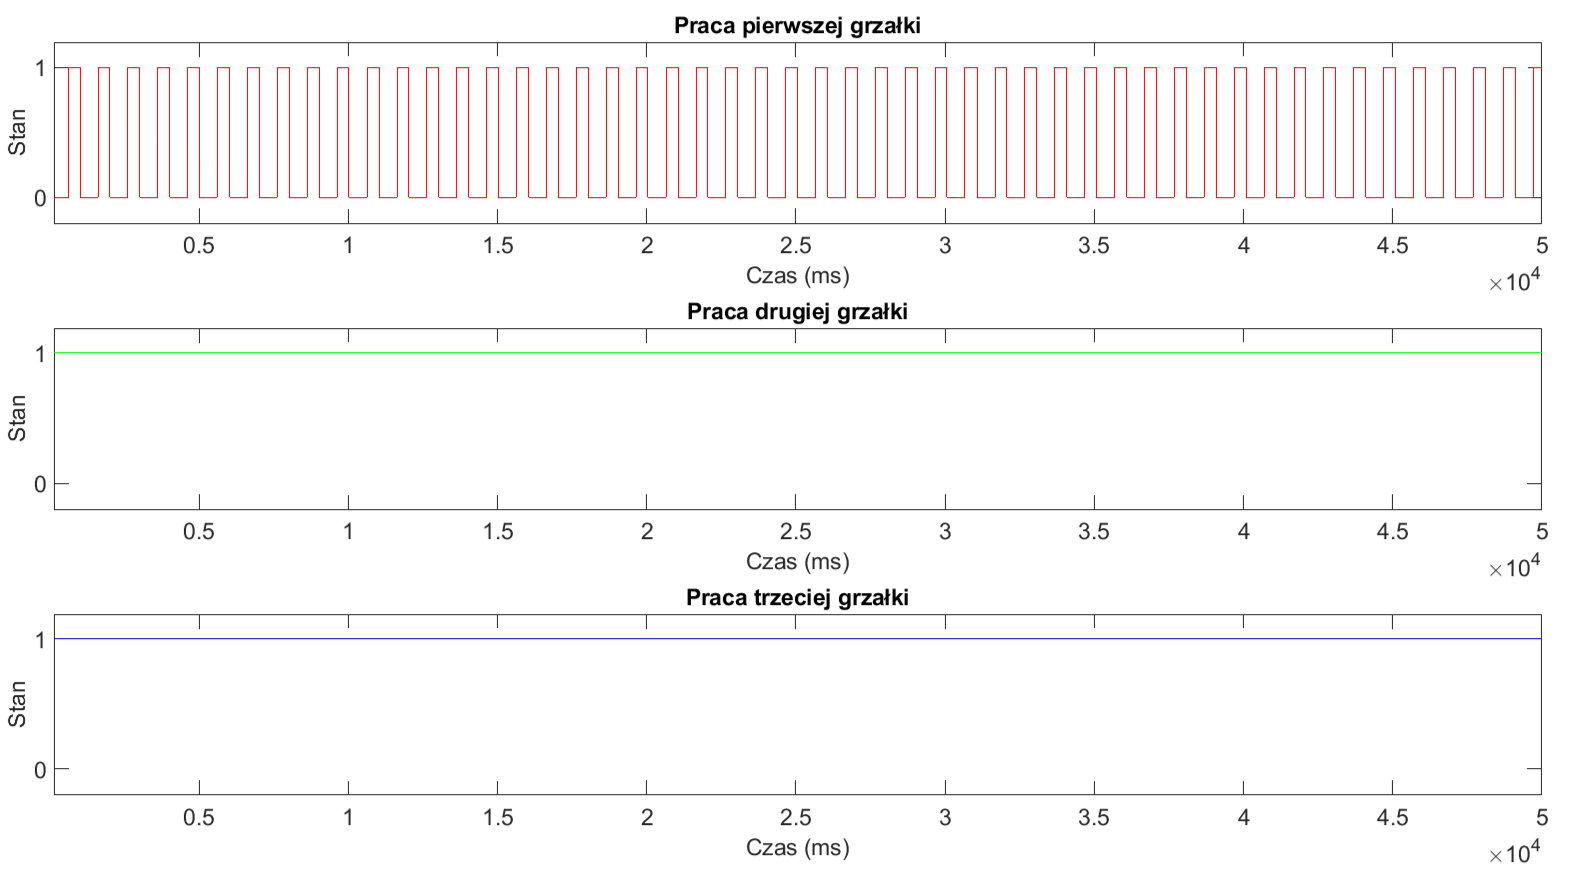
\includegraphics[width=0.92\textwidth]{./wykresy/png/threePhase80worse.png}
	\caption{Sterowanie trójfazowe (80\% mocy)}
	\label{fig:ThreePhase80worse}
\end{figure}

\noindent Praca na poziomie 80\% mocy wymaga przejścia dwóch grzałek w stały tryb pracy. Teraz, aktywnie przełączany jest wyłącznie przekaźnik grzałki pierwszej. Liczba przełączeń pierwszego przekaźnika osiągnęła wartość 598.

\subsubsection{Komentarz}
Niezależne sterowanie fazami, w sposób oczywisty, spowodowało nierównomierne rozłożenie pracy, pomiędzy poszczególnymi grzałkami. Pod tym względem, nastąpiło pogorszenie sterowania. W tym momencie, warto jednak zwrócić uwagę na to, że niezależnie od wartości zadanej użytkowej mocy pieca, zawsze tylko jedna z grzałek wymaga zmiennej pracy przekaźnika, który aby móc osiągnąć pożądaną moc skuteczną, musi być niesutannie przełączany. To powoduje, że główny cel algorytmu został już osiągnięty, ale wymaga kilku usprawnień, aby mógł być skutecznie implementowany i w pełni zastąpić klasyczne sterowanie, za pomocą trzech faz jednocześnie. Usprawnienie będzie polegało na dodaniu kilku modyfikacji, do istniejącego bloku \textit{ExecutePWM}.

\subsection{Modyfikacja bloku \textit{ExecutePWM}}

\begin{figure}[h]
	\centering
	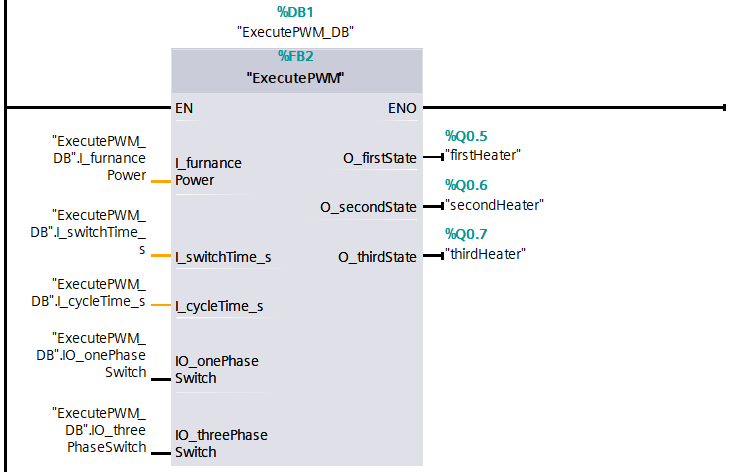
\includegraphics[width=0.8\textwidth]{./img/executePWMupdate.png}
	\caption{Zaktualizowany blok \textit{ExecutePWM}}
	\label{fig:ExecutePWM ulepszony}
\end{figure}

Do danych bloku dodane zostało wejście o nazwie \textit{I\_switchTime\_s (Real, s)}. Zmienna określa czas, po którym nastąpi zmiana obciążeń. Zmienne pomocnicze, przechowujące współczynniki wypełnienia PWM, nie zmienią wartości, ale zostaną przypisane do grzałek w innej konfiguracji, po upływie określonego czasu. Proces powtarza się cyklicznie. Po upływie trzech cykli przełączeniowych, dojdzie więc do wyrównania liczby przełączeń przekaźników oraz czasu pracy grzałek.

\newpage
\noindent Aktualne przypisanie odbywa się na podstaiwe numeru cyklu\(\ \in \{1, 2, 3\}\) (zmienna \textit{cycleCount, (Int)}). Możliwe przypadki przypisania realizowane są w fragmencie kodu języka SCL, zamieszczonego poniżej.\\

\begin{lstlisting}
IF #IO_threePhaseSwitch THEN
    CASE #cycleCount OF
        1:  
            #firstHeater := REAL_TO_INT(#firstFilling);
            #secondHeater := REAL_TO_INT(#secondFilling);
            #thirdHeater := REAL_TO_INT(#thirdFilling);
        2:  
            #firstHeater := REAL_TO_INT(#thirdFilling);
            #secondHeater := REAL_TO_INT(#firstFilling);
            #thirdHeater := REAL_TO_INT(#secondFilling);
        3:
            #firstHeater := REAL_TO_INT(#secondFilling);
            #secondHeater := REAL_TO_INT(#thirdFilling);
            #thirdHeater := REAL_TO_INT(#firstFilling);
    END_CASE;
END_IF;
\end{lstlisting}

\noindent Zmienna \textit{cycleCount} ulega zmianie zgodnie z następującym kodem LAD.

\begin{figure}[h]
	\centering
	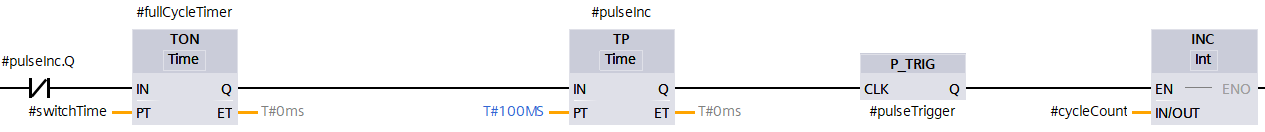
\includegraphics[width=1\textwidth]{./img/cycleCount.png}
	\caption{Zmiana wartości \textit{cycleCount}}
	\label{fig:CycleCount}
\end{figure}

\noindent Zegar \textit{TON} oznaczony jako \textit{fullCycleTimer} rozpoczyna odliczanie zadanego czasu jednego pełnego cyklu grzania, przechowywanego w zmiennej \textit{switchTime}. Po upłynięciu tego czasu, generowany jest pojedynczy impuls, oznaczony jako \textit{pulseInc (Int)}, który wyzwala blok \textit{INC}, pozwalający na inkrementację wartości \textit{cycleCount (Int)}. Zmienna \textit{cycleCount} informuje o tym, który z trzech przypadków przypisania (kod SCL), jest aktualnie realizowany. Wygenerowanie impulsu \textit{pulseInc} powoduje natychmiastowe zresetowanie zegara \textit{fullCycleTimer}. Cały proces powtarza się w sposób cykliczny, do momentu dezaktywacji trybu trójfazowego.

\newpage
\subsection{Cykliczne przełącznie grzałek}
Sposób przydzielania wypełnień nie ulega zmianie. Wartość zmiennej \textit{switchTime} ustalono na 100 s, co stanowi 1/3 czasu pełnego cyklu. Na finalnych przebiegach zostanie ujęty pełen, trzystusekundowy cykl pracy.

\begin{figure}[h]
	\centering
	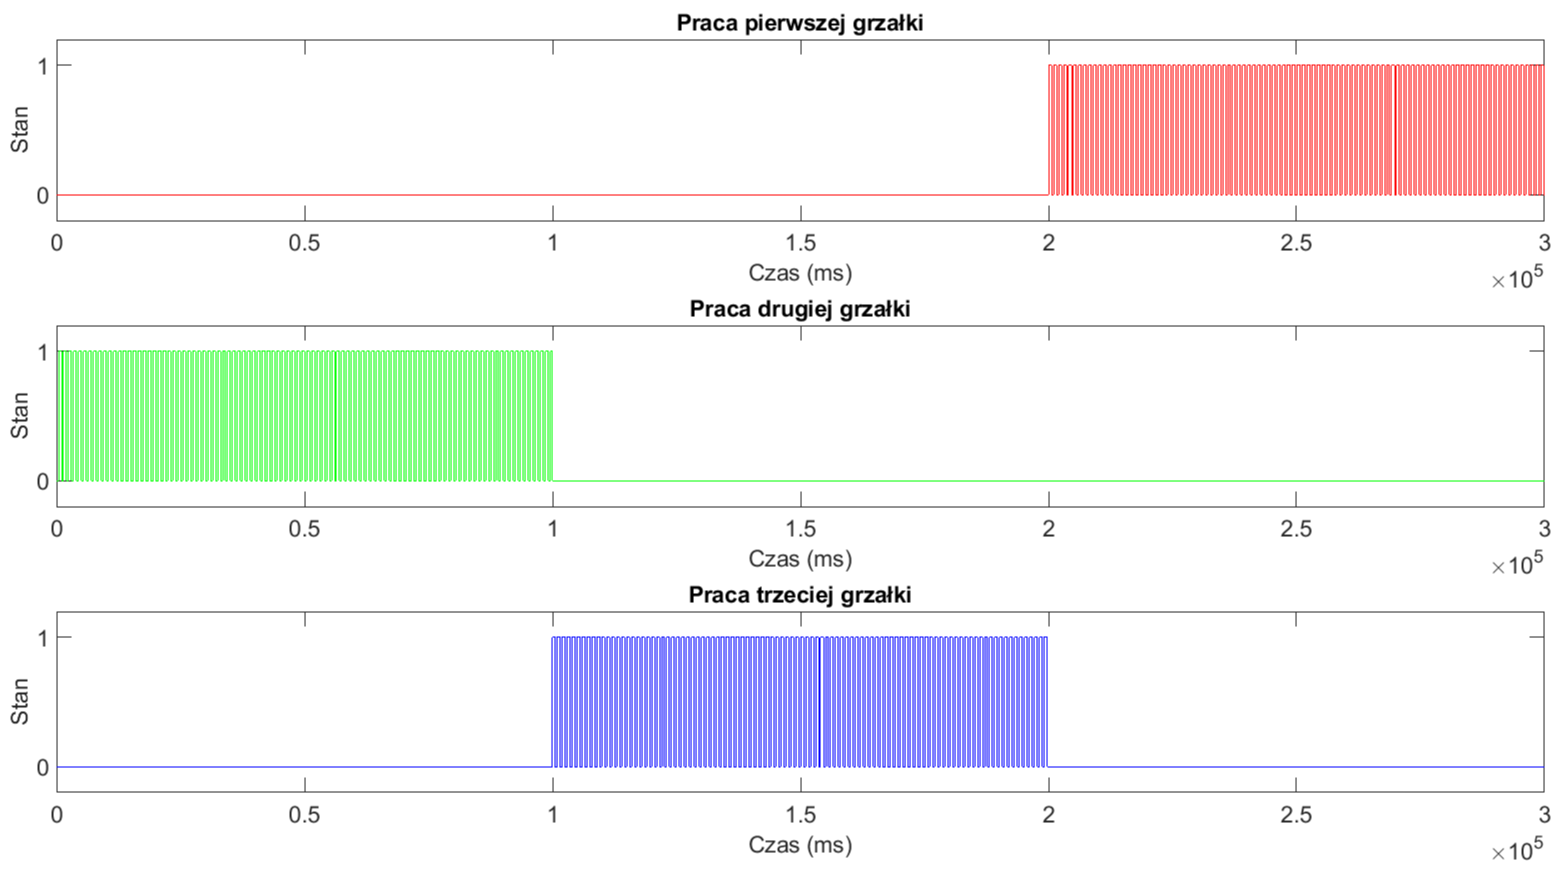
\includegraphics[width=0.94\textwidth]{./wykresy/png/threePhase20better.png}
	\caption{Usprawnione sterowanie trójfazowe (20\% mocy)}
	\label{fig:ThreePhase20better}
\end{figure}

\noindent Jak widać, co 100 s następuje zmiana obciążenia grzałek. Teraz, w trakcie trwania całego cyklu (300 s), do pojedynczej grzałki zostanie przpisane każde z obliczonych na początku wypełnień. Dzięki temu, niezależnie od zadanego obciążenia, każda grzałka wykona taką samą prace, po upływie trzech okresów określonych w \textit{switchTime}. Najłatwiej zauważyć to na przykładzie przegiegu z rys. 4.14. Na następnej stronie zamieszczono również wykresy dla 50\% i 80\% mocy zadanej.

\begin{figure}[h]
	\centering
	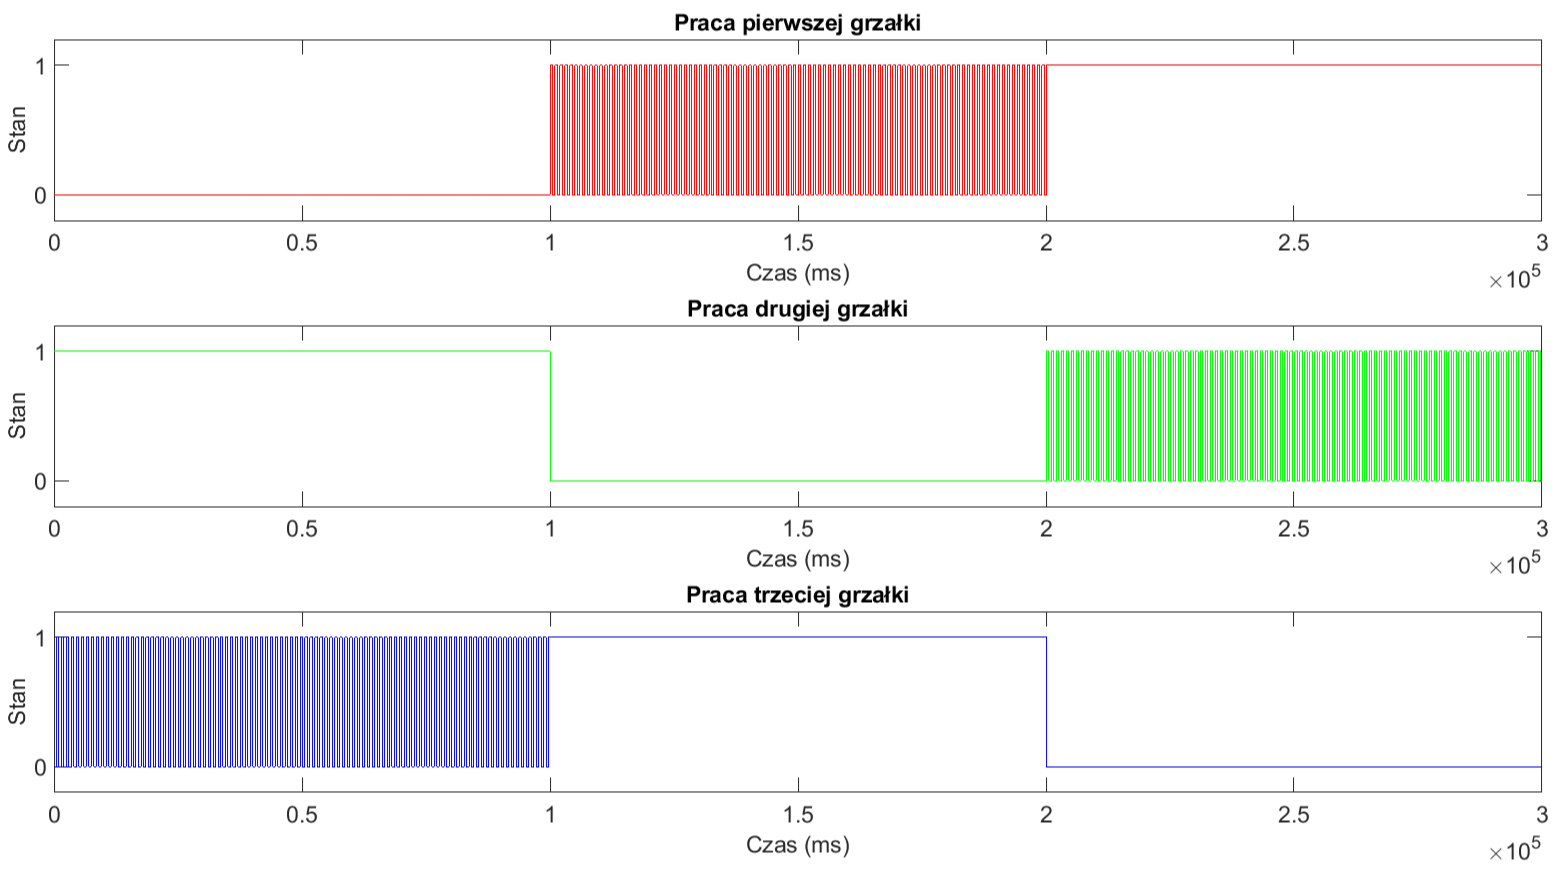
\includegraphics[width=0.94\textwidth]{./wykresy/png/threePhase50better.png}
	\caption{Usprawnione sterowanie trójfazowe (50\% mocy)}
	\label{fig:ThreePhase50better}
\end{figure}

\newpage
\begin{figure}[h]
	\centering
	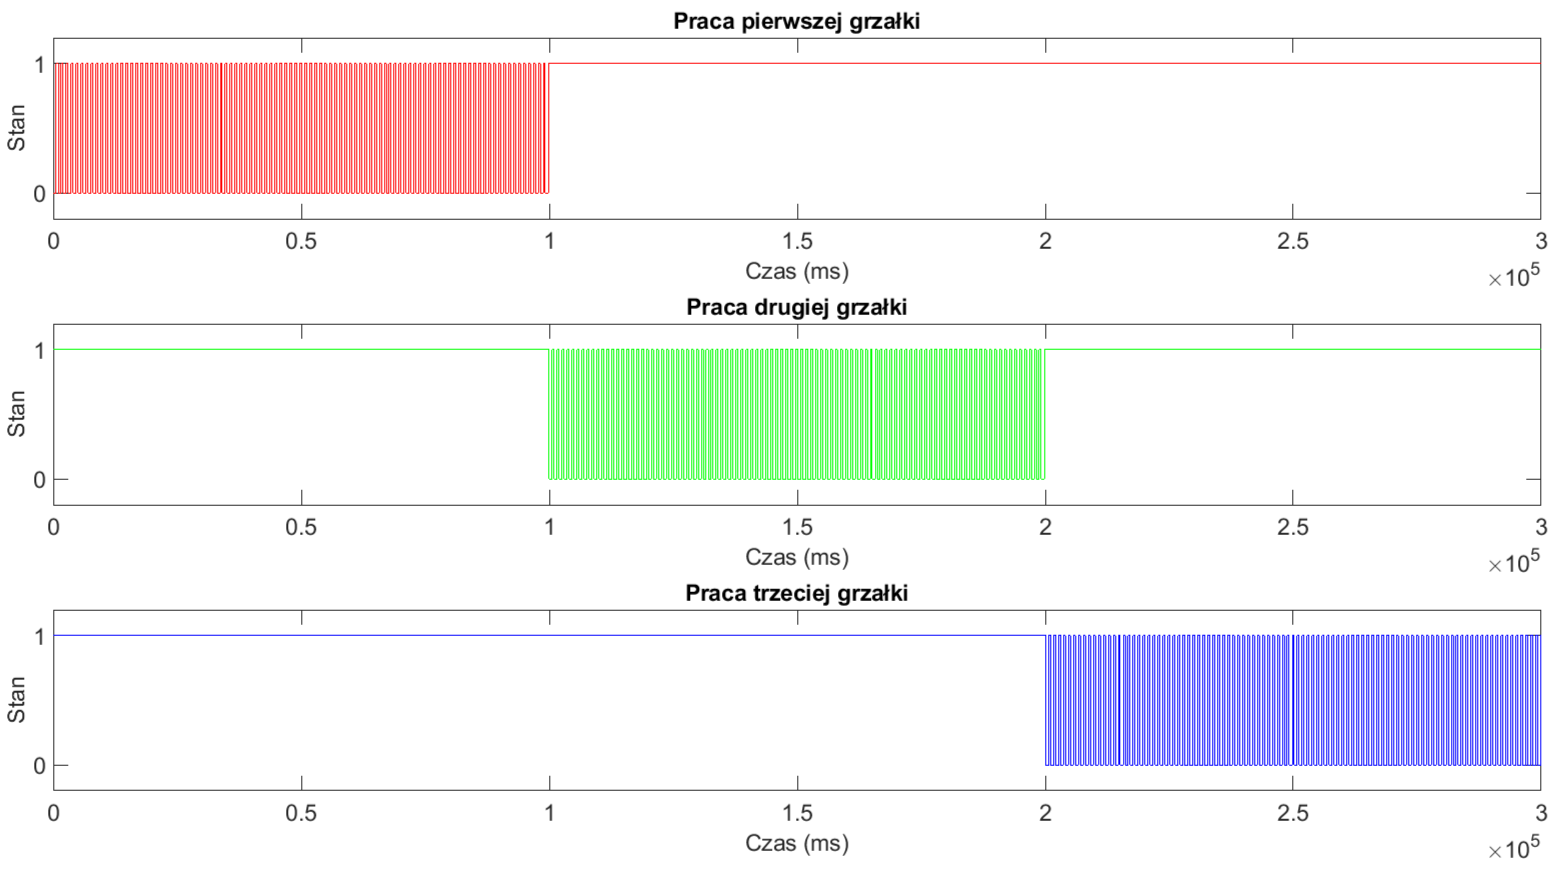
\includegraphics[width=0.94\textwidth]{./wykresy/png/threePhase80better.png}
	\caption{Usprawnione sterowanie trójfazowe (80\% mocy)}
	\label{fig:ThreePhase80better}
\end{figure}

\noindent W każdym okresie \textit{switchTime} aktywnie przełączany jest tylko jeden przekaźnik. Sumaryczna liczba przełączeń dla obciążeń 20\%, 50\%, 80\% wyniosła kolejno: 600, 606, 602.

\newpage

\subsection{Schemat blokowy}
W poprzednich rodziałach omówiono wyłącznie najważniejsze elementy programu, stworzonego na potrzeby tej pracy. Program pozwala na przełączanie sterowania pomiędzy trybami jednofazowym i trójfazowym, w dowolnym momencie. Zamieszczenie schematu blokowego pozwoli na ustystematyzowanie wszystkich kroków algorytmu.

\begin{figure}[h]
	\centering
	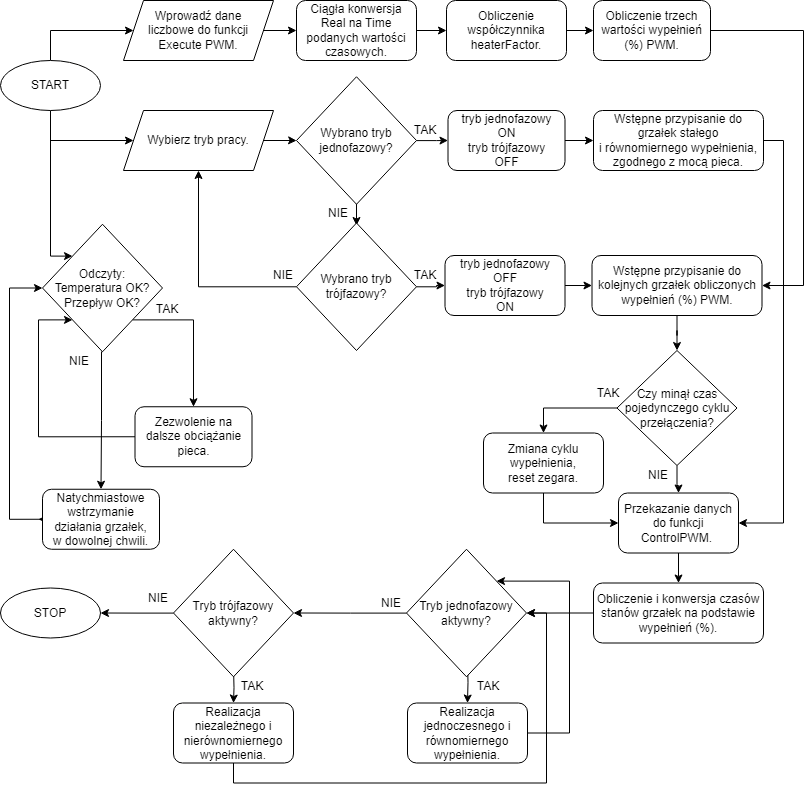
\includegraphics[width=1\textwidth]{./img/algorithm.png}
	\caption{Schemat blokowy algorytmu}
	\label{fig:Schemat blokowy}
\end{figure}

% TODO
\chapter{Konfiguracja instalacji}
\label{ch:05}
Rozpoczęcie pracy z instalacją wymaga odpowiedniego skonfigurowania komunikacji pomiędzy sterownikiem, a urządzeniami zgodnymi ze standardem IO-Link.

\subsection{Elementy systemu sterowania}
\subsubsection{Sterownik PLC SIMATIC 1516-3 PN/DP}
Sterownik umożliwia kontrolę procesów instalacji. Wyposażony jest w jednostkę centralną z 2 MB pamięci roboczej programu (RAM) i 5 MB na dynamiczne przechowywanie danych. Posiada 3 interfejsy komunikacyjne. Są to: PROFINET IRT (Isochronous Real-Time) z 2-portowym switchem, PROFINET RT (Real-Time) oraz PROFIBUS.

\begin{figure}[h]
	\centering
	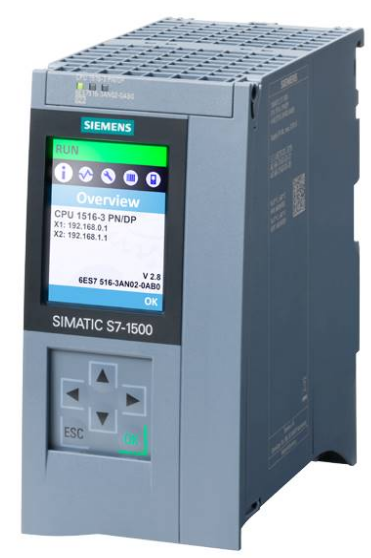
\includegraphics[width=0.20\textwidth]{./img/sterownik.png}
	\caption{Sterownik obecny w instalacji \cite{siemens}}
	\label{fig:Sterownik}
\end{figure}

\subsubsection{Moduł rozszerzeń wyjść cyfrowych SIMATIC DQ 32x24VDC/0,5A ST}
Standardowy moduł z rodziny roszerzeń ET 200MP, umożliwiających rozbudowę funkcjonalności sterownika. Moduł przeznaczony jest do obsługi dodatkowych 32 wyjść cyfrowych, o napięciu 24V DC i maksymalnym prądzie wyjściowym.

\newpage
\subsubsection{Moduł rozszerzeń wejść analogowych SIMATIC AI 8xU/I/RTD/TC ST}
Inny moduł standardowy z rodziny roszerzeń ET 200MP, który służy do rozbudowy funkcjonalności obsługi wejść analogowych. Moduł wyposażono w osiem kanałów, mogących odbierać zarówno sygnały prądowe jak i napięciowe. Dodatkowo, możliwa obsługa sygnałów z termopar(TC) i rezystancyjnych czujników temperatury (RTD).

\subsubsection{Moduł rozszerzeń wyjść analogowych SIMATIC  AQ 4xU/I ST}
Standardowy moduł wyposażony w 4 kanały, które służą do generowania sygnałów analogowych, w celu sterowania urządzeniami, wymagającymi ciągłej regulacji sygnału.

\begin{figure}[h]
	\centering
	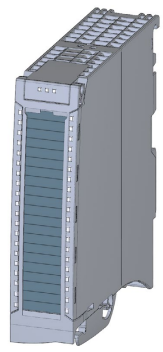
\includegraphics[width=0.20\textwidth]{./img/module.png}
	\caption{Wygląd modułów rozszerzeń \cite{siemens}}
	\label{fig:Moduł cyfrowy}
\end{figure}

\begin{figure}[h]
	\centering
	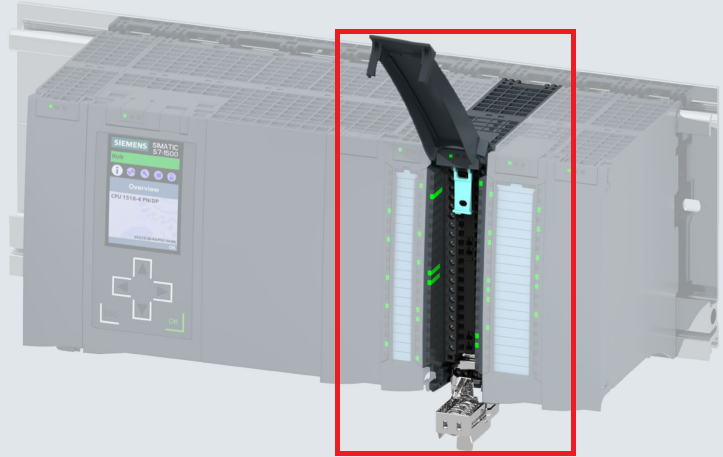
\includegraphics[width=0.8\textwidth]{./img/multiModule.png}
	\caption{Sposób montażu dodatkowych modułów \cite{siemens}}
	\label{fig:Sposób montażu}
\end{figure}

\subsection{Standard IO-Link}
\subsubsection{Moduł Master IO-Link IFM AL1102 z interfejsem PROFINET}
IO-Link to standard komunikacji w przemyśle, który pozwala na komunikację dwukierunkową, pomiędzy urządzeniami pomiarowymi (sensorami), a systemem sterowania. Słowo "master" oznacza, że moduł pełni rolę głównego urządzenia, zarządzającego komunikacją z sensorami IO-Link. Zastosowanie modułu umożliwia konfigurację urządzeń pomiarowych, z poziomu sterownika oraz przesyłanie danych diagnostycznych, co wpływa pozytywnie na uporządkowanie sensorów oraz łatwość wprowadzania potencjalnych modyfikacji w instalacji. Moduł jest odporny na pył oraz wilgoć zgodnie ze standardem IP67. Moduł konfiguruje się poprzez wykorzystanie plików GSDML.

\begin{figure}[h]
	\centering
	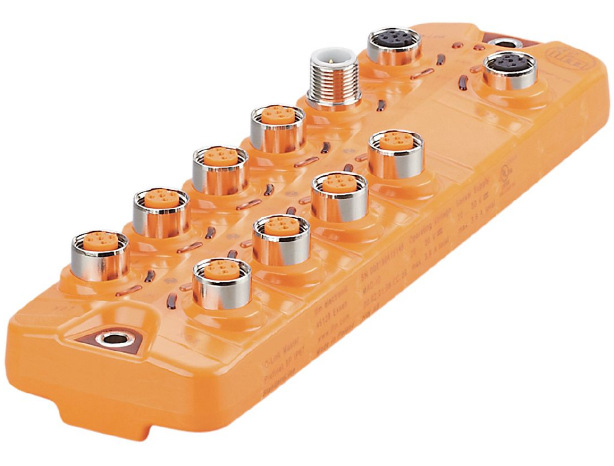
\includegraphics[width=0.6\textwidth]{./img/IOLink.png}
	\caption{Moduł IO-Link obecny w instalacji \cite{ifm}}
	\label{fig:Moduł IO-Link}
\end{figure}

\noindent Do modułu podłącza się sensory zgodne ze standardem IO-Link. Przykładowe sensory producenta IFM Electronic obecne w instalacji to: presostat PP7554, czujnik temperatury TA2417, przepływomierz elektromagnetyczny SM6100.

\begin{figure}[h]
	\centering
	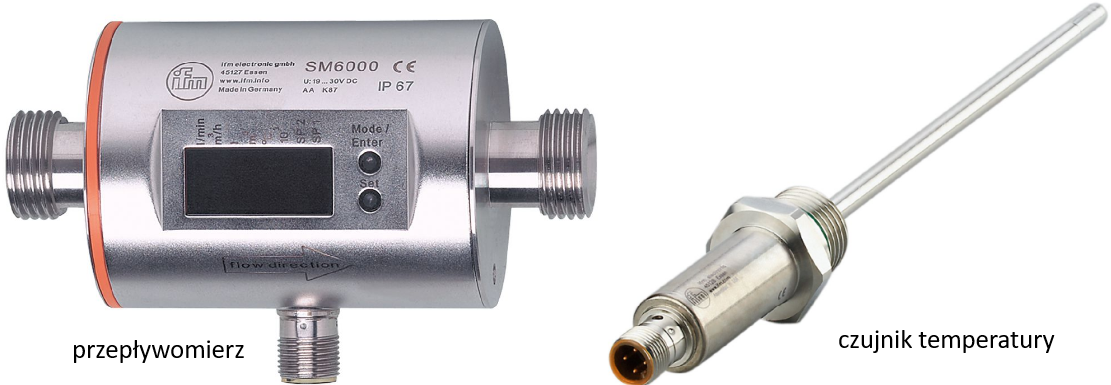
\includegraphics[width=0.65\textwidth]{./img/sensory.png}
	\caption{Sensory IO-Link \cite{ifm}}
	\label{fig:Sensory IO-Link}
\end{figure}

\newpage
\subsection{Zabezpieczenia}
Kod programu zawiera w sobie zabezpieczenia, które umożliwiają prawidłowe działanie algorytmu oraz wpływają pozytywnie na bezpieczeństwo pracy z instalacją. Zabezpieczenia obejmują:
\begin{itemize}
	\item Brak możliwości uruchomienia obu trybów sterowania jednocześnie.
	\item Natychmiastowe wyłączenie wszystkich grzałek, gdy przepływ nie mieści się w określonych granicach bezpieczeństwa (0.5 l/min - 10 l/min) lub temperatura na wyjściu jest zbyt wysoka (> 70\textdegree{}C).
	\item Natychmiastowe wyzerowanie sygnałów, jeżeli żaden z trybów sterowania nie jest aktywny.
\end{itemize}

\begin{figure}[h]
	\centering
	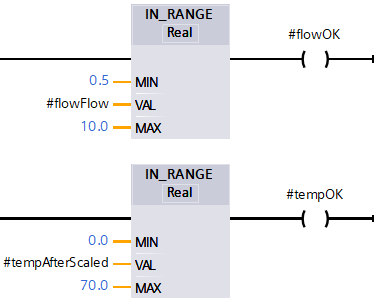
\includegraphics[width=0.4\textwidth]{./img/safety1.png}
	\caption{Kontrola parametrów}
	\label{fig:Kontrola parametrów}
\end{figure}

\begin{figure}[h]
	\centering
	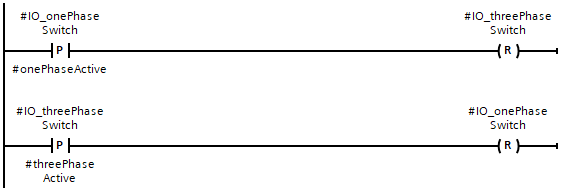
\includegraphics[width=0.7\textwidth]{./img/safety2.png}
	\caption{Dezaktywacja jednego z trybów}
	\label{fig:Dezaktywacja trybu}
\end{figure}

\begin{figure}[h]
	\centering
	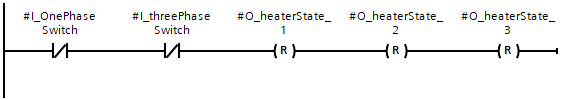
\includegraphics[width=0.7\textwidth]{./img/safety3.png}
	\caption{Wyłączenie pieca}
	\label{fig:Wyłączenie pieca}
\end{figure}

% TODO
\chapter{Weryfikacja i walidacja na rzeczywistym układzie regulacji}
\label{ch:06}
Rozdział dotyczy omówienia procesu implementacji algorytmu, na instalacji cieplnej, obecnej na wydziale AEI Politechniki Śląskiej. Analiza zebranych danych umożliwi porównanie przedstawionych metod sterowania, pod kątem regulacji rzeczywistego układu.

\subsection{Aktualizacja programu}

\begin{figure}[h]
	\centering
	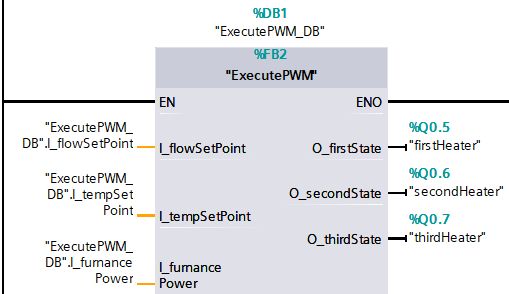
\includegraphics[width=0.7\textwidth]{./img/executePWMrelugation.png}
	\caption{Zaktualizowany blok \textit{ExecutePWM}}
	\label{fig:Aktualizacja funkcji ExecutePWM}
\end{figure}

Funkcja \textit{ExecutePWM} została uaktualniona o wejścia \textit{I\_flowSetPont (Real, l/min)} oraz \textit{I\_tempSetPoint (Real, \textdegree{}C)}. Zmienne reprezentują wartości zadane przepływu oraz temperatury, które zostaną przekazane jako parametry wejściowe, do bloku technologicznego \textit{PID\_Compact}, dostępnego w środowisku TIA Portal.

\newpage
Instrukcje \textit{PID\_Compact} zostały umieszczone w bloku organizacyjnym o nazwie \textit{Cyclic interrupt}. Blok pozwala na realizację cyklicznego przerwania, które umożliwia skoordynowane i powtarzalne wykonywanie zadań w czasie rzeczywistym, niezależnie od głównego bloku programu \textit{Main}. Cykl przerwania regulacji temperatury oraz przepływu został ustalony na czas 100 ms.\\

Podczas wykonywania pomiarów, przepływ będzie zmieniany wyłącznie raz z wartości 2 l/min do 2,5 l/min, a jego niewielkie wahania są akceptowalne. Bardziej istotna, w kontekście porównania sposóbów sterowania, jest regulacja temperatury cieczy przepływającej przez piec. Proces doboru jak najlepszych nastaw regulatora, będzie więc skupiony wyłącznie wokół regulacji temperatury.

\begin{figure}[h]
	\centering
	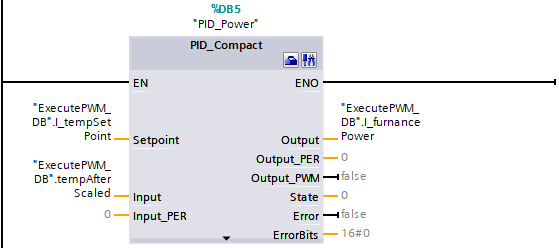
\includegraphics[width=0.8\textwidth]{./img/PID_Compact.png}
	\caption{Blok technologiczny \textit{PID\_Compact} sterujący mocą zadaną}
	\label{fig:PID_Compact}
\end{figure}

\noindent Powyższy blok korzysta wyłącznie ze sparametryzowanych wartości zmiennych. Wejście i wyjście oznaczone jako \textit{\_PER} pozostają więc nieaktywne (służą do odczytu danych bezpośrednio z urządzeń pomiarowych). Regulator PID steruje mocą pieca, w zależności od temperatury zadanej oraz przeskalowanego odczytu z czujnika temperatury, na wyjściu pieca.

\subsection{Proces regulacji}
Dla wszystkich sposobów doboru nastaw, pomiar trwa 14 min. Zmiana temperatury następuje co 2 min, w następującej sekwencji:\\
\noindent 30\textdegree{}C $\rightarrow$ 40\textdegree{}C $\rightarrow$ 20\textdegree{}C $\rightarrow$ 30\textdegree{}C $\rightarrow$ 40\textdegree{}C $\rightarrow$ 20\textdegree{}C $\rightarrow$ 30\textdegree{}C.\\
\noindent Zmiana przepływu z wartości 2 l/min na 2,5 l/min następuje po upływie około 6 min.

\subsubsection{Domyślne parametry środowiska TIA Portal}
Pierwsze testy zostały przeprowadzone dla domyślnych parametrów regulatora.\\Wartości nastaw są następujące: \textit{kr} = 1, \textit{T$_i$} = 20, \textit{T$_d$} = 0.

\newpage
\begin{figure}[h]
	\centering
	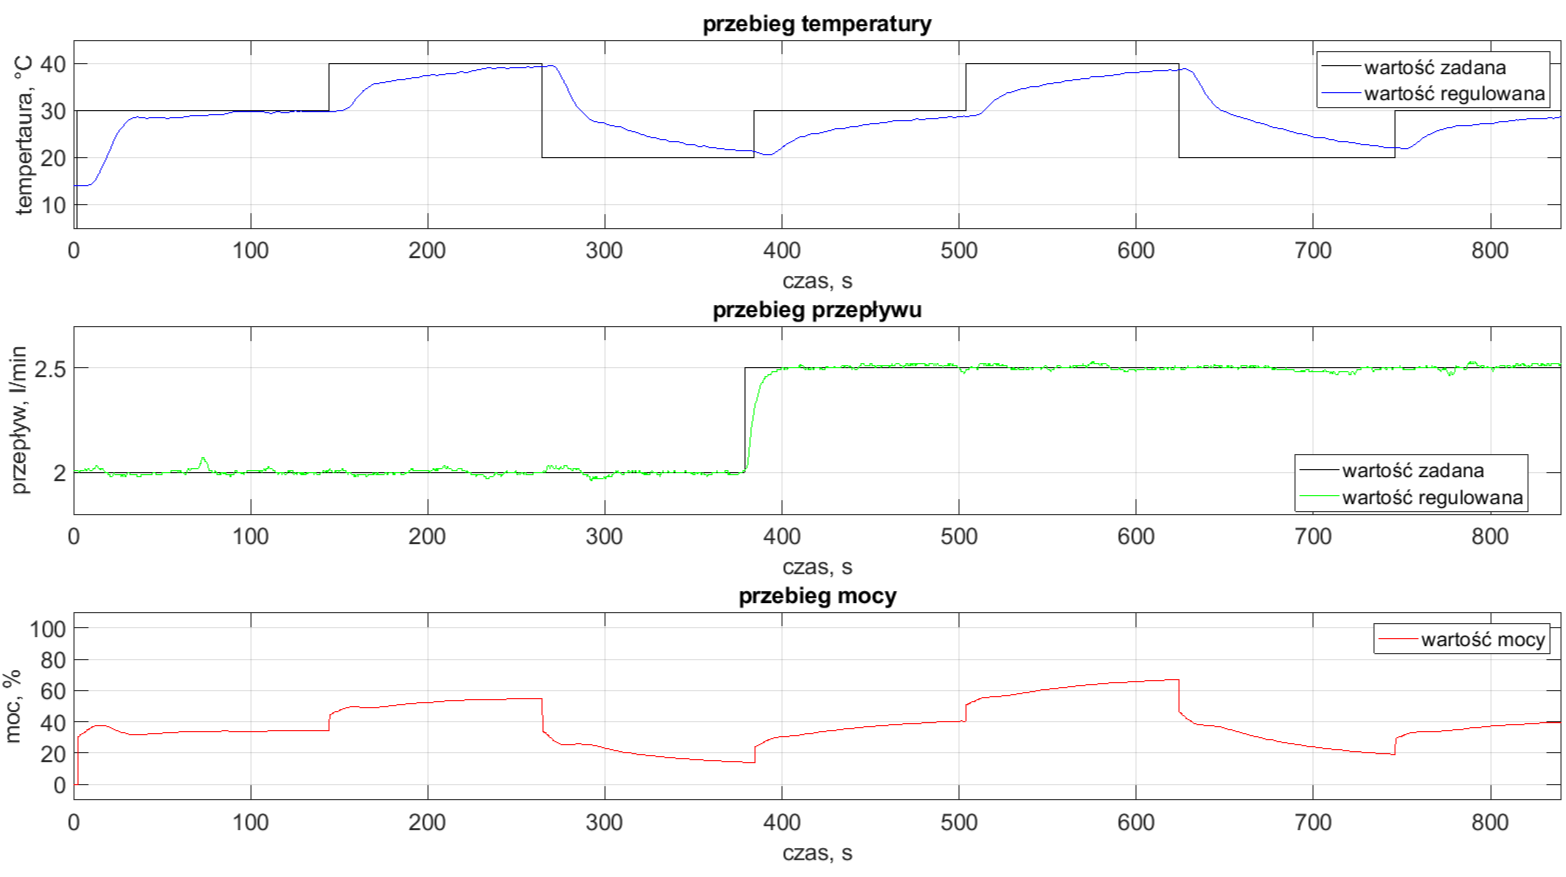
\includegraphics[width=0.92\textwidth]{./wykresy/png/regulation(default)OnePhase.png}
	\caption{Przebieg regulacji sterowania jednofazowego (nastawy domyślne)}
	\label{fig:Jednofazowe domyślne}
\end{figure}

\begin{figure}[h]
	\centering
	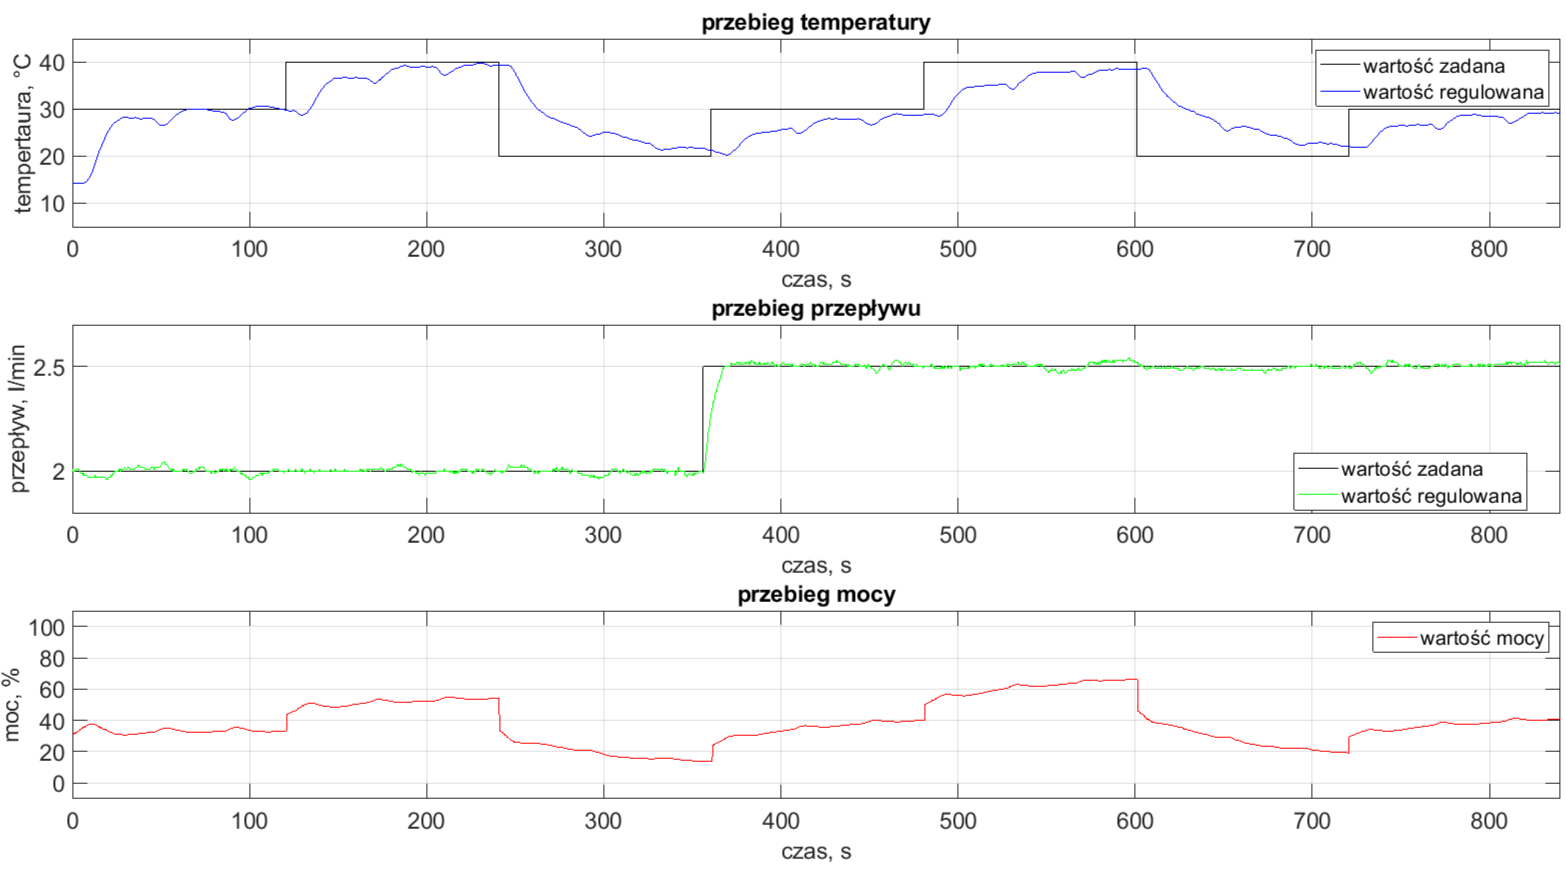
\includegraphics[width=0.92\textwidth]{./wykresy/png/regulation(default)ThreePhase.png}
	\caption{Przebieg regulacji sterowania trójfazowego (nastawy domyślne)}
	\label{fig:Trójfazowe domyślne}
\end{figure}

\subsubsection{Komentarz}
Na podstawie przebigów można ocenić, że regulacja nie działa w zadowalający sposób. Aby uzyskać miarodajne porównania sposobów sterowania, konieczne będzie zoptymalizowanie nastaw regulatora PID.

\newpage
\subsubsection{Metoda dwóch punktów}
Metoda została zaprezentowana podczas jednego z laboratoriów, na przedmiocie Podstawy Automatyki, realizowanego w ramach kierunku Automatyka i Robotyka, na Politechnice Śląskiej. Metoda opiera się na doborze dwóch punktów \textit{(t, y)}, na podstawie odpowiedzi skokowej układu. Punkty stanowią momenty czasu \textit{t}, w których odpowiedź skokowa układu osiąga 28,3\% oraz 63,2\% stanu ustalonego \textit{y}. Na podstawie wyznaczonych czasów \textit{t} można dokonać estymacji następujących parametrów transmitancji:\\

\textbf{stała czasowa inercji pierwszego rzędu}
\begin{equation}
	T = 1,5 (t_2 - t_1)
\end{equation}

\textbf{czas opóźnienia}
\begin{equation}
	T_O = t_1 - T
\end{equation}

\textbf{wzmocnienie układu}
\begin{equation}
	k = \frac{\Delta y}{\Delta u}
\end{equation}

\noindent Parametry obliczone za pomocą metody dwóch punktów można następnie wykorzystać w ramach kryteriów strojenia regulatorów, na przykład kryterium Zieglera-Nicholsa \cite{ziegler1942optimum}, znanego również jako kryterium QDR.\\

\noindent W celu wyznaczenia odpowiedzi skokowej instalacji cieplnej, dokonano nagłej zmiany mocy pieca z wartości 0\% do 100\%, przy stałym przepływie wynoszącym 2,25 l/min. Odpowiedź (temperaturę wyjściową) monitorowano przez 2 min.

\begin{figure}[h]
	\centering
	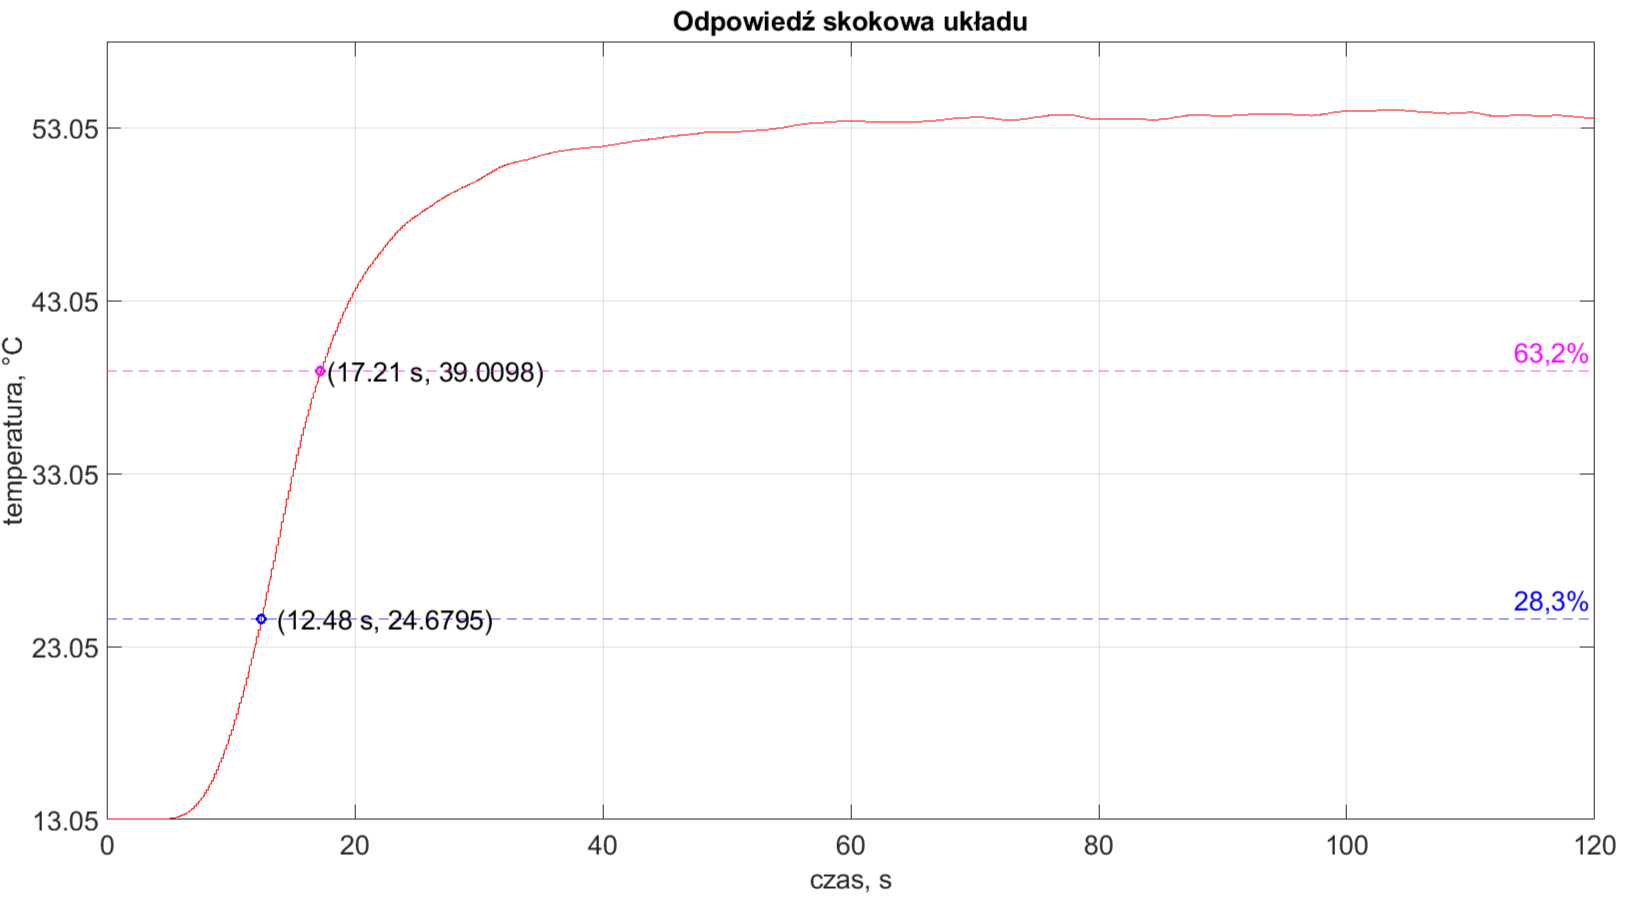
\includegraphics[width=0.92\textwidth]{./wykresy/png/stepResponse.png}
	\caption{Odpowiedź skokowa układu}
	\label{fig:Odpowiedź skokowa}
\end{figure}

\newpage
\noindent Na wykresie zaznaczono liniami przerywanymi wartości 28,3\% (granatowy) oraz 68,2\% (fioletowy) stanu ustalonego. Współrzędne \textit{t} punktów oraz obliczone na ich podstawie stałe czasowe wyniosły około:
\textit{$t_1$} = 12,48 s, \textit{$t_2$} = 17,21 s, \textit{T} = 7,10 s, \textit{$T_O$} = 10,12 s. Wzmocnienie układu \textit{k} = 0,41.\\

Czas opóźnienia instalacji wyniósł ponad 10 s, ponieważ układy cieplne charakteryzują się sporym opóźnieniem. Ponadto, czas opóźnienia $T_O$ jest większy od stałej czasowej \textit{T}, przez co proces regulacji układu może być problematyczny. Przykładowym kryterium, przeznaczonym dla układów o dużym opóźnieniu, jest kryterium Cohena-Coona, będące modyfikacją nastaw kryterium Zieglera-Nicholsa.

\subsubsection{Kryterium Cohena-Coona, \cite{cohen1953theoretical}}
\begin{table}[h]
	\centering
	\caption{Nastawy kryterium Cohena-Coona}
	\label{id:tab:Cohen Conn}
	\renewcommand\cellalign{lc} % Wyrównanie komórek
	\setcellgapes{2.0ex} % Dodatkowy odstęp w komórkach

	\makegapedcells % Zastosowanie dodatkowego odstępu
	\begin{tabular}{|c|c|c|c|c|}
		\hline
		parametr & $\alpha$                                    & $k_r$                                                           & $T_I$                                       & $T_D$ \\
		\hline
		wzór     & $\frac{T_O}{T}$                             & $\frac{T}{{k T_O}} \left(\frac{4}{3} + \frac{\alpha}{4}\right)$ & $T_O \frac{{32 + 6\alpha}}{{13 + 8\alpha}}$
		         & $T_O \frac{{32 + 6\alpha}}{{13 + 8\alpha}}$
		\\
		\hline
		wartość  & 1,43                                        & 2,89                                                            & 16,81                                       & 2,92  \\
		\hline
	\end{tabular}
\end{table}

\noindent Nastawy obliczone w ten sposób, pozwalają uzyskać przebiegi przedstawione na dwóch kolejncyh rysunkach.

\begin{figure}[h]
	\centering
	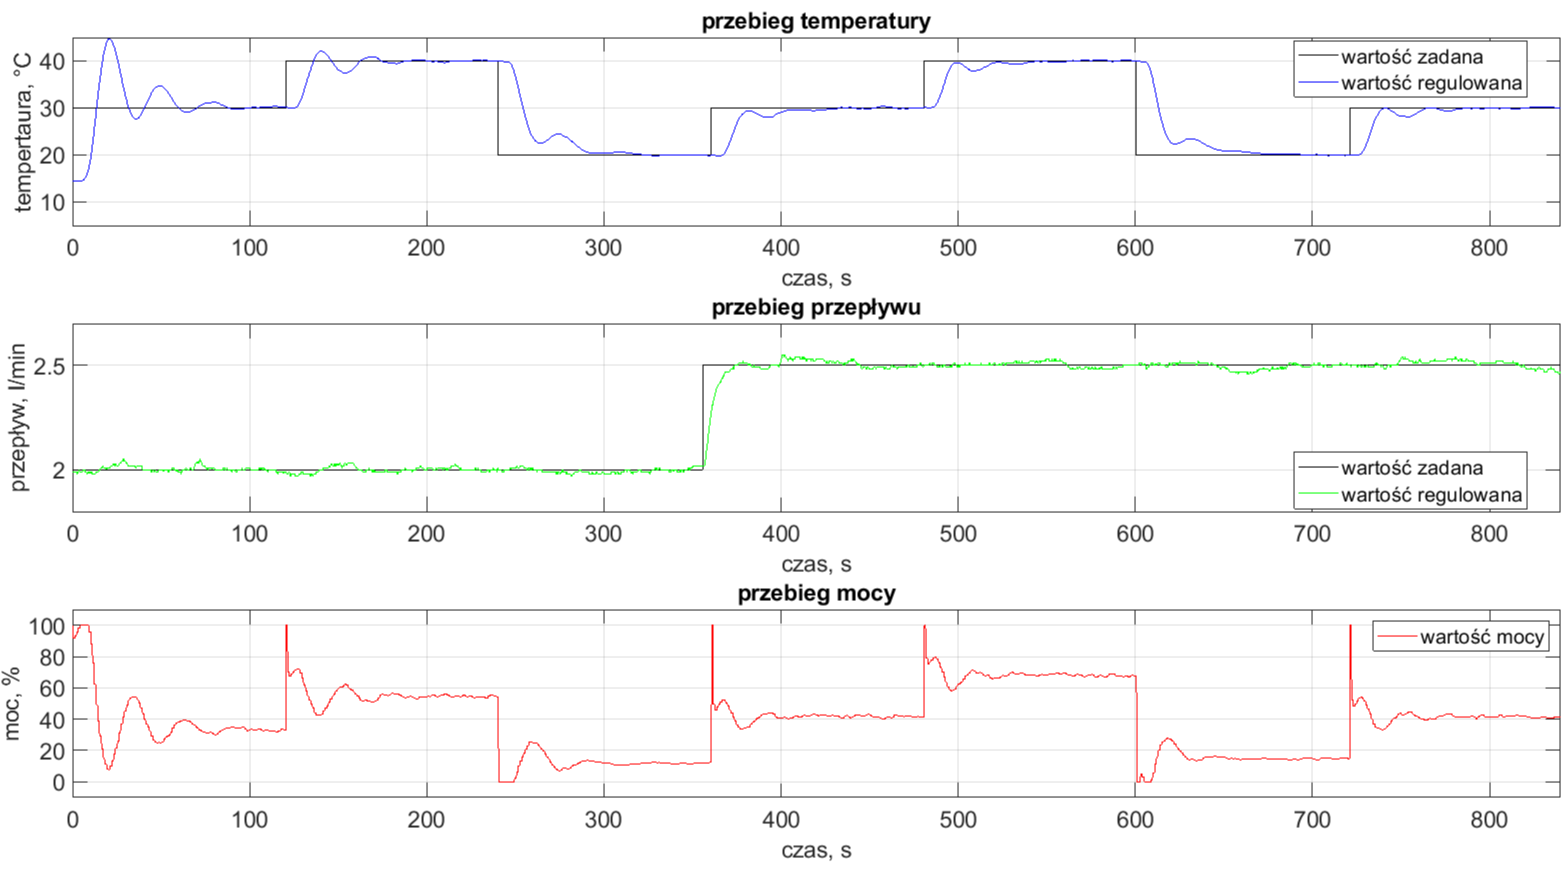
\includegraphics[width=0.92\textwidth]{./wykresy/png/regulation(CohenCoon)OnePhase.png}
	\caption{Przebieg regulacji sterowania jednofazowego (kryterium Cohena-Coona)}
	\label{fig:Cohen Coon jednofazowy}
\end{figure}

\newpage
\begin{figure}[h]
	\centering
	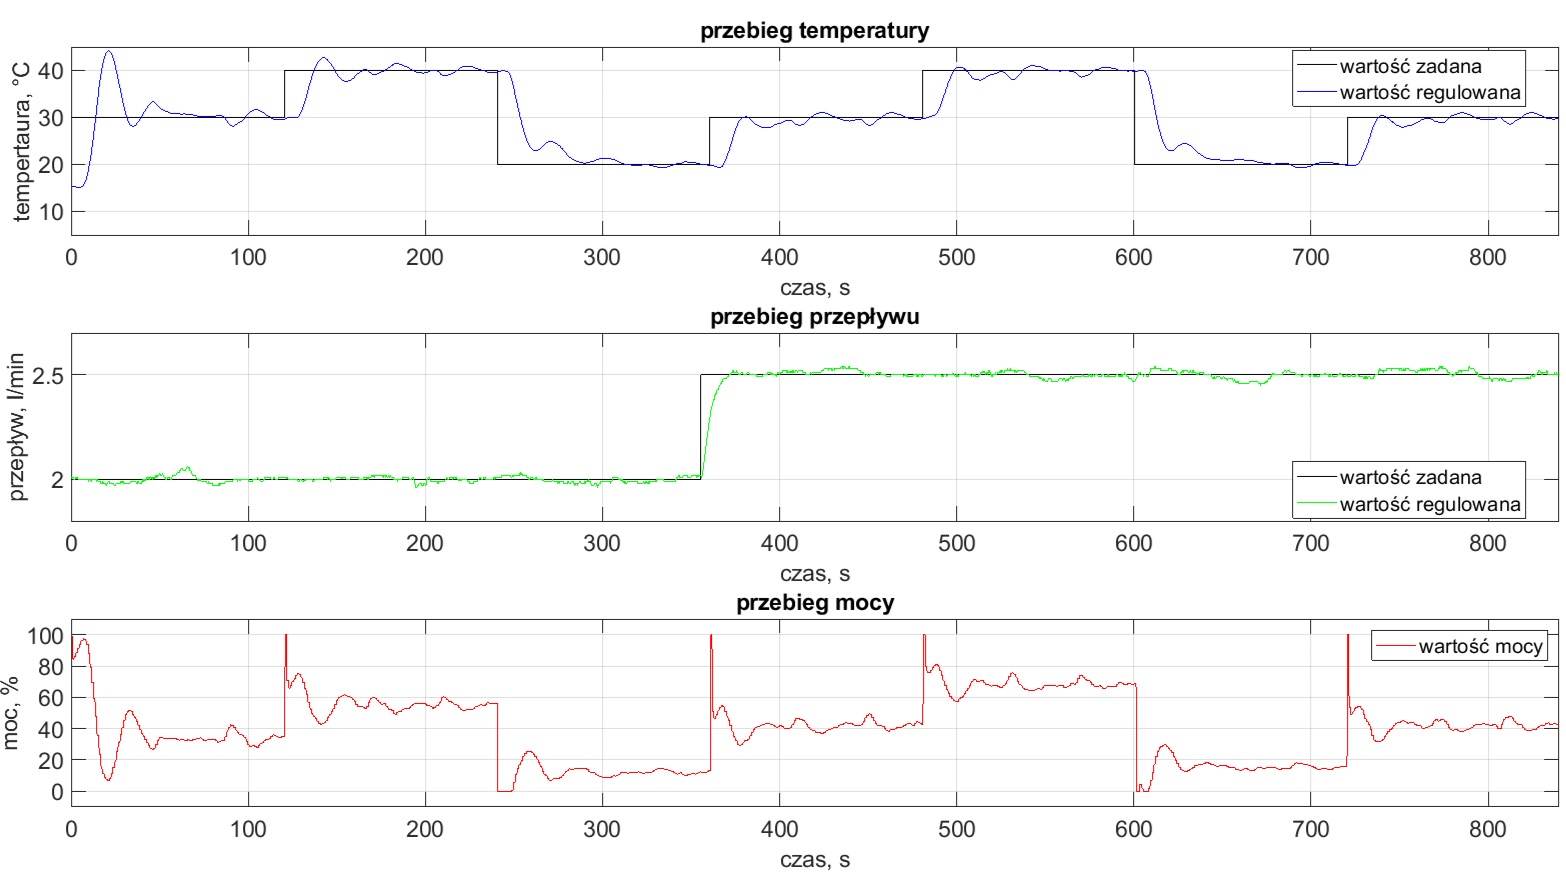
\includegraphics[width=0.92\textwidth]{./wykresy/png/regulation(CohenCoon)ThreePhase.png}
	\caption{Przebieg regulacji sterowania trójfazowego (kryterium Cohena-Coona)}
	\label{fig:Cohen Coon trójfazowy}
\end{figure}

\subsubsection{Komentarz}
Zgodnie z oczekiwaniami, regulacja PID uległa znacznej poprawie. Warto również zwrócić uwagę na to, że w jednofazowym modelu sterowania, wystąpiły znacznie mniejsze wahania temperatury, pomimo faktu, że w piecu obecne są trzy identyczne grzałki. Następny wykres pomoże zrozumieć powody, dla których wystąpiły różnice w działaniu prezentowanych trybów sterowania.

\begin{figure}[h]
	\centering
	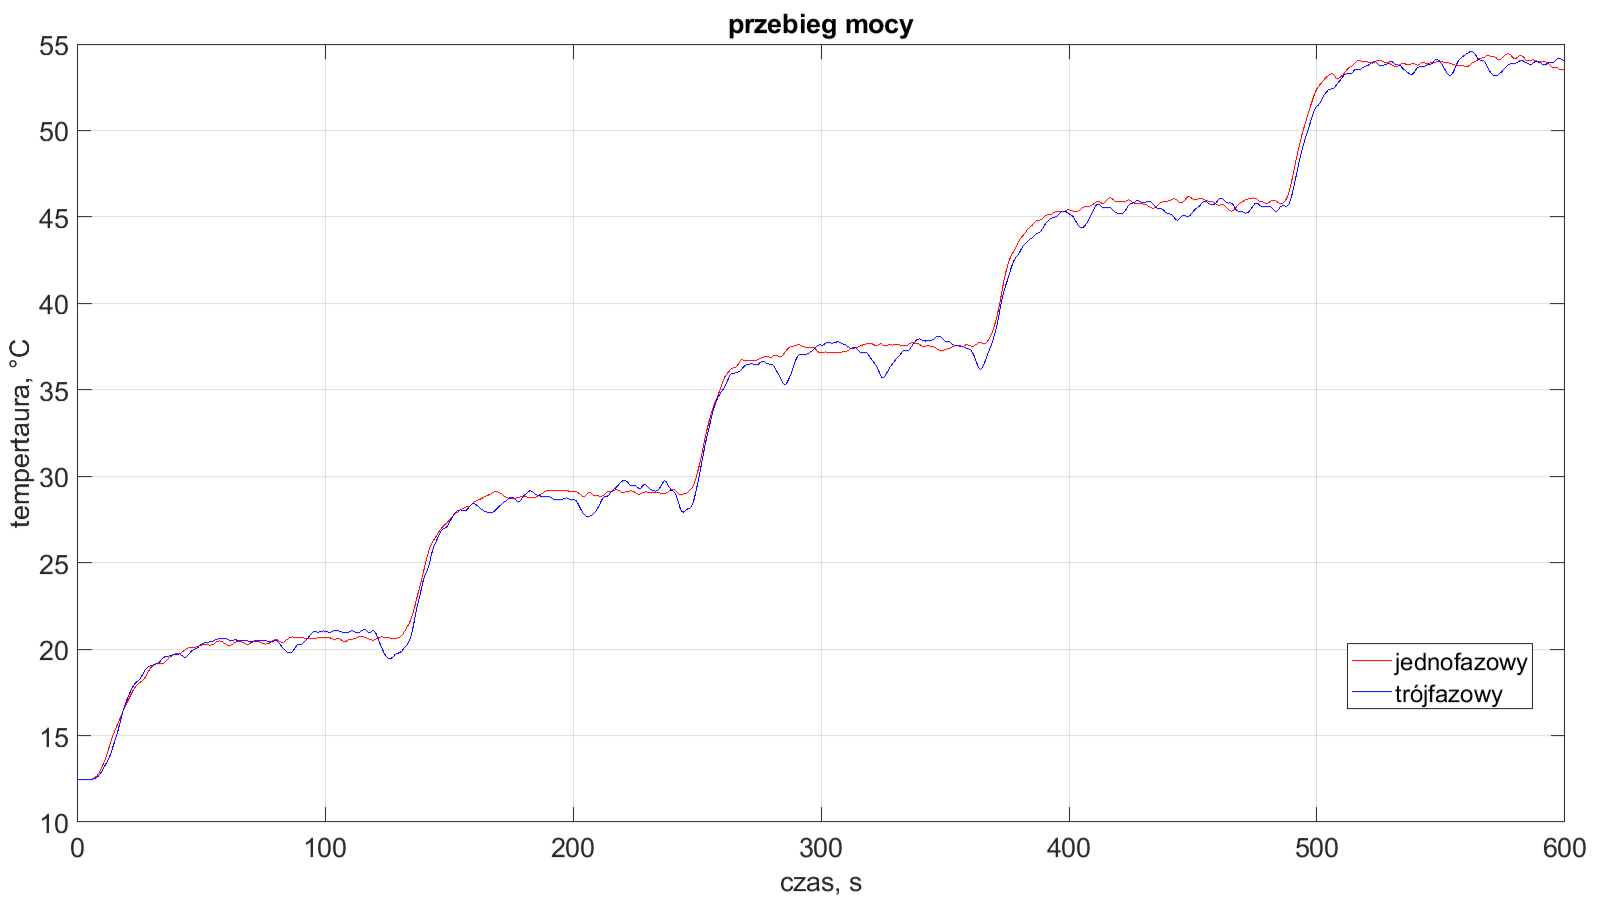
\includegraphics[width=0.92\textwidth]{./wykresy/png/stepCompare.png}
	\caption{Zestawienie wykresów odpowiedzi układu na skokowe zmiany mocy}
	\label{fig:Wykresy mocy}
\end{figure}

\newpage
\noindent Wykres z rys. 6.8 przedstawia zmiany temperatury, przy dwudziestoprocentowych skokach mocy, dla sterowania jednofazowego (czerwony) i trójfazowego (granatowy), zestawione na jednym wykresie. Skoki mocy realizowane są co 2 min, wobec czego czas cyklu pomiędzy przełączeniem grzałek wynosi 40 s (1/3 czasu interwału). Jak widać, temperatura przy sterowaniu jednofazowym, utrzymuje się na bardziej stabilnym poziomie, podczas gdy w trybie trójfazowym, można co jakiś czas zaobserwować niewielkie jej spadki. \\

Warto zauważyć, że spadki temperatury pokrywają się z cyklami zmian obciążenia grzałek. Wynika to głównie z faktu, że dopiero uruchomiona grzałka potrzebuje chwili, aby się zagrzać. Efekt ten jest najprawdopodobniej zauważalny w mniejszym stopniu, gdy grzałka pracuje w trybie stałym, dlatego największe różnice uwydatniają się w środkowym przedziale mocy, gdzie udział wypełnienia PWM jest największy. Drugim powodem tego stanu rzeczy jest nierównomierne rozłożenie ciepła w piecu, podczas sterowania fazami osobno. Strumień wody może bowiem w zmienny sposób opływać każdą z grzałek, w różnych chwilach czasu.\\

Oba te problemy nie występują podczas sterowania jednofazowego, gdyż zarówno praca grzałek, jak i geometryczne ich rozmieszczenie, jest w tym przypadku równomierne.\\

W obu przypadkach wartości temperatury nie odbiegają znacząco od wartości zadanej, więc jakość procesu można uznać za dobrą. Nagła zmiana mocy nie sprzyja regulacji w trybie trójfazowym. Przebieg temperatury mógłby ulec poprawie, gdyby zmiana mocy była stopniowa i rozpoczynała się odpowiednio wcześniej (przed momentem całkowitej zmiany obciążenia). Takie rozwiązanie wykracza jednak poza zakres tej pracy.

\subsubsection{Kryterium ISE \cite{soni2013bf}}
Celem kryterium jest minimalizacja całkowitej sumy kwadratów błędów (uchybu). Stosując kryterium jakości ISE (ang. integral of squared error) oczekuje się likwidacji przeregulowania, co powinno prowadzić do minimalizowania oscylacji.

\begin{table}[h]
	\centering
	\caption{Nastawy kryterium ISE}
	\label{id:tab:ISE}
	\renewcommand\cellalign{lc}
	\setcellgapes{2.0ex}

	\makegapedcells % Zastosowanie dodatkowego odstępu
	\begin{tabular}{|c|c|c|c|}
		\hline
		parametr & $k_r$                  & $T_I$    & $T_D$    \\
		\hline
		wzór     & $1,4 \frac{T}{{kT_O}}$ & $1,3T_O$ & $0,5T_O$
		\\
		\hline
		wartość  & 2,39                   & 13,15    & 5,06     \\
		\hline
	\end{tabular}
\end{table}

\begin{figure}[h]
	\centering
	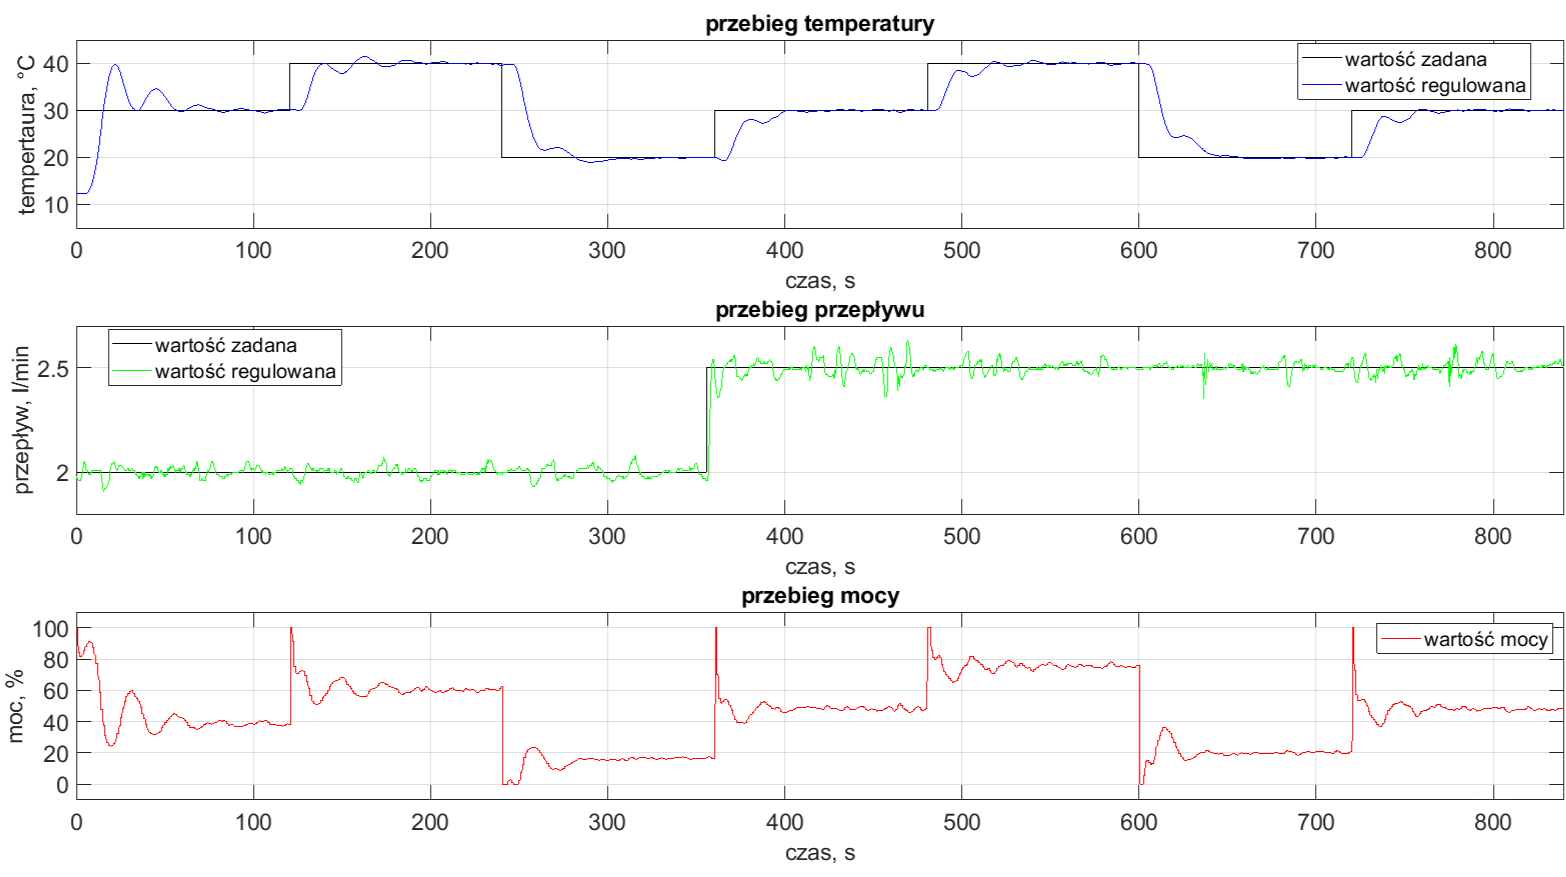
\includegraphics[width=0.92\textwidth]{./wykresy/png/regulation(ISE)OnePhase.png}
	\caption{Przebieg regulacji sterowania jednofazowego (kryterium ISE)}
	\label{fig:ISE jednofazowy}
\end{figure}

\newpage
\begin{figure}[h]
	\centering
	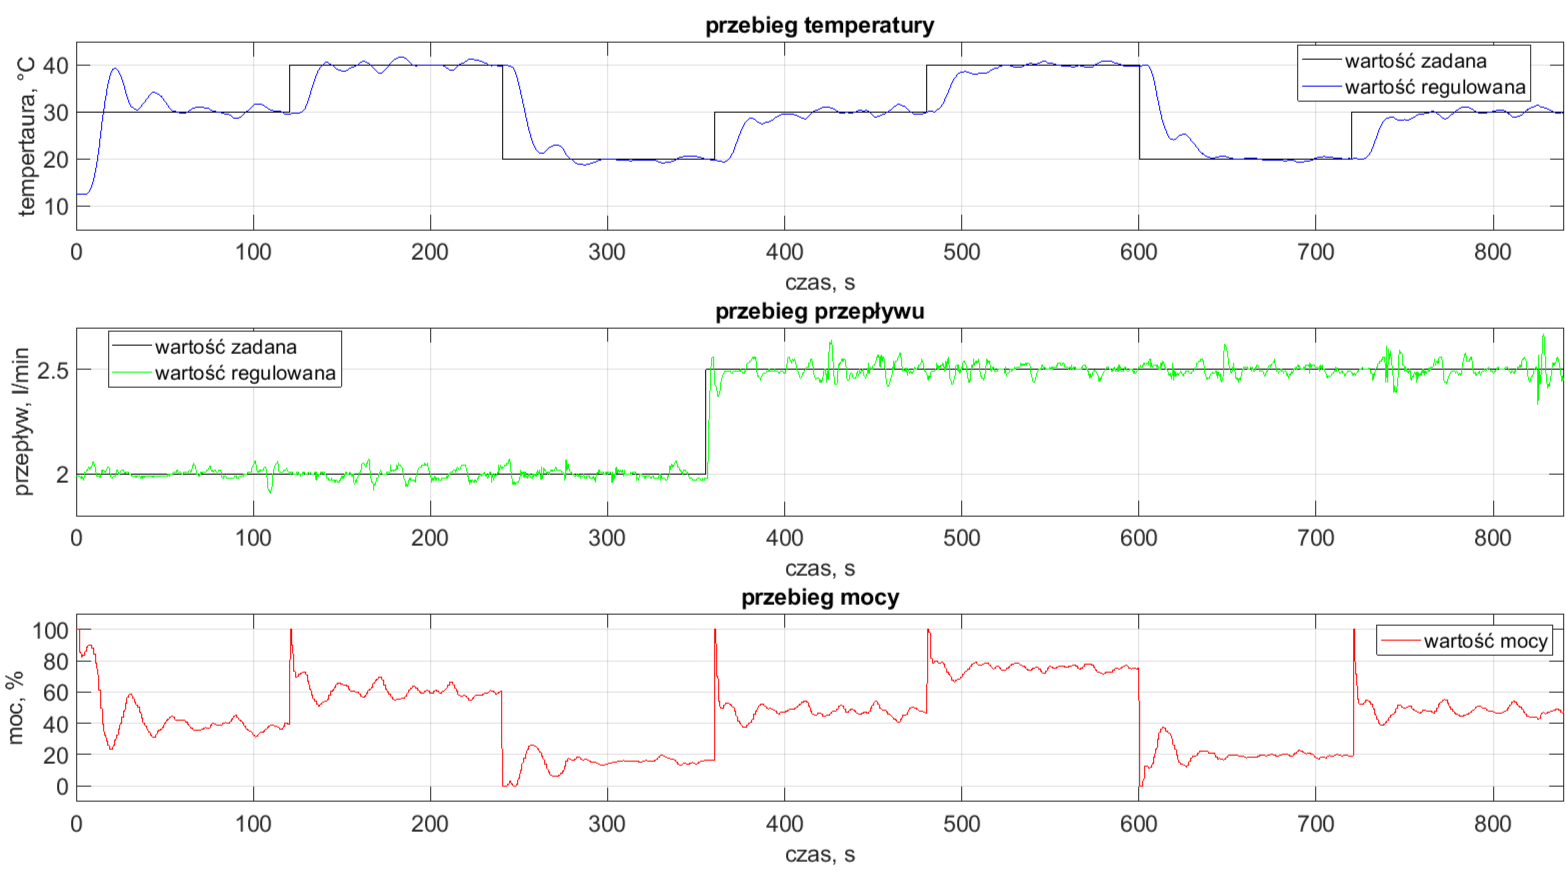
\includegraphics[width=0.92\textwidth]{./wykresy/png/regulation(ISE)ThreePhase.png}
	\caption{Przebieg regulacji sterowania trójfazowego (kryterium ISE)}
	\label{fig:ISE trójfazowy}
\end{figure}

\subsubsection{Komentarz}
W obu przypadkach nastąpiła nieznaczna poprawa regulacji, jednak regulator w dalszym ciągu działa lepiej podczas jednofazowego sterowania grzałkami.

% TODO
\chapter{Podsumowanie i wnioski}
\label{ch:07}
Algorytm realizujący niezależne sterowanie grzałkami działa poprawnie. Program napisany w środowisku TIA Portal oraz praca na układzie regulacji, pozwoliła na miarodajne porównanie wyników, które zostaną podsumowane w tym rozdziale. Zestawienie wyników pozwoli na wyciągnięcie wniosków, dotyczących różnych aspektów efektywności, zaprezentowanych podejść do sterowania układem.

\subsection{Podsumowanie wyników}
\begin{table}[h]
	\centering
	\caption{Tabela podsumowująca wyniki}
	\label{tab:example}
	\begin{tabular}{|c|c|c|c|c|c|c|c|c|c|c|c|c|c|}
		\hline
		\multicolumn{2}{|c}{}                                              & \multicolumn{4}{|c|}{SJF} & \multicolumn{4}{c|}{STF(A)} & \multicolumn{4}{c|}{STF(B)}                                                                                         \\
		\hline
		\multicolumn{2}{|c|}{MZP, \%}                                      & 20                        & 50                          & 80                          & $\sum$ & 20                    & 50   & 80  & $\sum$ & 20  & 50  & 80  & $\sum$       \\
		\hline
		\parbox[t]{2mm}{\multirow{3}{*}{\rotatebox[origin=c]{90}{LPP}}}    & G1                        & 599                         & 598                         & 599    & 1796                  & 599  & 0   & 0      & 599 & 200 & 201 & 200    & 601 \\
		\cline{2-14}
		                                                                   & G2                        & 598                         & 598                         & 599    & 1795                  & 0    & 600 & 0      & 600 & 200 & 202 & 202    & 604 \\
		\cline{2-14}
		                                                                   & G3                        & 599                         & 598                         & 599    & 1796                  & 0    & 0   & 598    & 598 & 200 & 203 & 200    & 603 \\
		\hline
		\multicolumn{2}{|c|}{$\sum_{\text{LPP}}$}                          & \multicolumn{3}{|c|}{}    & 5387                        & \multicolumn{3}{c|}{}       & 1797   & \multicolumn{3}{c|}{} & 1808                                                 \\








		\hline
		\parbox[t]{2mm}{\multirow{3}{*}{\rotatebox[origin=c]{90}{CPG, s}}} & G1                        & 60                          & 150                         & 240    & 450                   & 180  & 300 & 300    & 780 & 60  & 150 & 240    & 450 \\
		\cline{2-14}
		                                                                   & G2                        & 60                          & 150                         & 240    & 450                   & 0    & 150 & 300    & 450 & 60  & 150 & 240    & 450 \\
		\cline{2-14}
		                                                                   & G3                        & 60                          & 150                         & 240    & 450                   & 0    & 0   & 120    & 120 & 60  & 150 & 240    & 450 \\
		\hline
		\multicolumn{2}{|c|}{$\sum_{\text{CPG}}$}                          & \multicolumn{3}{|c|}{}    & 1350                        & \multicolumn{3}{c|}{}       & 1350   & \multicolumn{3}{c|}{} & 1350                                                 \\
		\hline
	\end{tabular}
\end{table}

\noindent Opis oznaczeń:
\begin{description}
	\item[\textbf{MZP}:]moc zadana pieca, \%
	\item[\textbf{LPP}:]liczba przełączeń przekaźnika
	\item[\textbf{CPG}:]czas pracy grzałki, s
	\item[\textbf{SJF}:]sterowanie jednofazowe
	\item[\textbf{STF(A)}:]sterowanie trójfazowe, wersja bez zmiany obciążenia
	\item[\textbf{STF(B)}:]sterowanie trójfazowe, wersja ze zmianą obciążenia
\end{description}

\newpage
\subsection{Wnioski}
Równy czas włączenia grzałek oznacza wykonanie przez nie podobnej pracy, czyli zbliżoną ilość energii cieplnej, oddanej do układu. Taki sposób zestawienia wyników pozwoli na porównanie działania sposobów sterowania, przy podobnej efektywności układu. Jak widać w tabeli 7.1, porównanie liczby przełączeń przekaźników jest realizowane na podstawie identycznego sumarycznego czasu ich włączenia, wynoszącego około 1350 s.

\subsubsection{Sterowanie jednofazowe}
Liczba przełączeń przekaźników jest w tym trybie około trzykrotnie większa, niż w przypadku sterowania trójfazowego. Uzyskane przebiegi temperatury utrzymują wartości na bardzo stabilnym poziomie, dzięki czemu łatwo dobrać nastawy regulatora, które skutkują wysoką wydajnością energetyczną.

\subsubsection{Sterowanie trójfazowe}
Ten sposób sterowania układem powoduje, że w krótkich chwilach czasu następuje nierównomierne rozłożenie energii w piecu, w związku z czym występują niewielkie wahania temperatury wyjściowej. Efektem jest otrzymanie układu, którego praca jest trudniejsza do wyregulowania, jednak dzięki sterowaniu trzema fazami osobno, zdołano zmniejszyć liczbę przełączeń przekaźników aż trzykrtonie, co znacząco przełoży się na zminimalizowanie ich zużycia.

\subsubsection{Komentarz końcowy}
Jeżeli układ wymaga bardzo precyzyjnej regulacji temperatury, lepszym wyborem będzie sterowanie jednofazowe, które pozwoli na równomierną i efektywną wymianę ciepła. Jeżeli jednak wahania temperatury są akcpetowalne, w określonych granicach tolerancji, lepiej zdecydować się na sterowanie trójfazowe, gdyż działanie usparwnionego algorytmu w minimalizuje zużycie przekaźników w znaczącym stopniu.

\backmatter

\printbibliography
\addcontentsline{toc}{chapter}{Bibliografia}
\label{ch:08}

\begin{appendices}

	% TODO
	\chapter{Spis skrótów i symboli}

	\begin{itemize}
		\item[$PWM$] (ang. \english{Pulse-Width Modulation}) modulacja szerokości impulsu
		\item[$ISE$] (ang. \english{integral of squared error}) całka z kwadratu błędu
		\item[$QDR$] (ang. \english{quarter decay ratio}) współczynnik rozpadu kwartalnego
		\item[$SCL$] (ang. \english{structure control language}) strukturalny język programowania
		\item[$LAD$] (ang. \english{ladder logic}) graficzny język programowania
		\item[$TON$] (ang. \english{timer on delay}) typ timera dostępnego w środowisku TIA Portal
		\item[$K(s)$] transmitancja dziedziny operatorowej
		\item[$SJF$] sterowanie jednofazowe
		\item[$STF$] sterowanie trójfazowe
		\item[$MZP$] moc zadana pieca
		\item[$LPP$] liczba przełączeń przekaźnika
		\item[$CPG$] czas pracy grzałki
		\item[$PID$] typ regulatora (ang. \english{proportional-integral-derivative})
		\item[$\in$] przynależność do zbioru wartości
		\item[$\notin$] wykluczenie ze zbioru wartości
		\item[l] (jednostka objętości) litr
		\item[min] (jednostka czasu) minuta
	\end{itemize}
	Pozostałe oznaczenia są zgodne z układem SI.

	% TODO
	\chapter{Lista dodatkowych plików, uzupełniających tekst pracy}
	\label{ch:09}

	\textbf{Do pracy dołączono dodatkowe pliki zawierające:}
	\begin{itemize}
		\item algorytm stworzony w środowisku TIA Portal V17 (.zap17)
		\item dane pomiarowe z instalacji cieplnej (.csv)
		\item dane pomiarowe dostosowane do odczytu (.xslx)
		\item pliki prezentujące sposób przetwarzania wykresów przy użyciu środowiska Matlab (.m)
		\item wygresy wygenerowane w środowisku Matlab (.fig)
		\item dokumnetację konfiguracyjną oraz pomoce naukowe (.pdf)
		\item schematy blokowe, narysowane za pomocą internetowego narzędzia \href{https://app.diagrams.net/}{diagrams.net} (.drawio)
	\end{itemize}

	\listoffigures
	\addcontentsline{toc}{chapter}{Spis rysunków}
	\listoftables
	\addcontentsline{toc}{chapter}{Spis tabel}

\end{appendices}

\end{document}

%% Finis coronat opus.